% mn2esample.tex
%
% v2.1 released 22nd May 2002 (G. Hutton)
%
% The mnsample.tex file has been amended to highlight
% the proper use of LaTeX2e code with the class file
% and using natbib cross-referencing. These changes
% do not reflect the original paper by A. V. Raveendran.
%
% Previous versions of this sample document were
% compatible with the LaTeX 2.09 style file mn.sty
% v1.2 released 5th September 1994 (M. Reed)
% v1.1 released 18th July 1994
% v1.0 released 28th January 1994


\documentclass[useAMS,usenatbib]{mn2e}
\usepackage{graphicx}
\usepackage{float}

% If your system does not have the AMS fonts version 2.0 installed, then
% remove the useAMS option.
%
% useAMS allows you to obtain upright Greek characters.
% e.g. \umu, \upi etc.  See the section on "Upright Greek characters" in
% this guide for further information.
%
% If you are using AMS 2.0 fonts, bold math letters/symbols are available
% at a larger range of sizes for NFSS release 1 and 2 (using \boldmath or
% preferably \bmath).
%
% The usenatbib command allows the use of Patrick Daly's natbib.sty for
% cross-referencing.
%
% If you wish to typeset the paper in Times font (if you do not have the
% PostScript Type 1 Computer Modern fonts you will need to do this to get
% smoother fonts in a PDF file) then uncomment the next line
% \usepackage{Times}

%%%%% AUTHORS - PLACE YOUR OWN MACROS HERE %%%%%


%%%%%%%%%%%%%%%%%%%%%%%%%%%%%%%%%%%%%%%%%%%%%%%%

\title[Young protoplanetary discs]{Simulated observations of young protoplanetary discs}
%authors arent splitting over 2 lines so rawlings is pushed off the edge
\author[Tom Douglas, Paola Caselli, Et al.]{Tom Douglas$^{1}$\thanks{E-mail:
pytd@leeds.ac.uk}, Paola Caselli$^{1}$, Aaron Boley$^{2}$, Richard Durisen$^{3}$, Tom Hartquist$^{1}$, John Ilee$^{1}$, Jonathon Rawlings$^{4}$ \\
$^{1}$School of Physics and Astronomy, University of Leeds, Leeds LS2 9JT, UK \\
$^{2}$Department of Astronomy, University of Florida, 211 Bryant Space Center, PO Box 112055, USA\\
$^{3}$Department of Astronomy, Indiana University, 727 East 3rd Street, Swain West 319, Bloomington, IN 47405, USA\\
%$^{4}$Department of Physics & Astronomy, University College London, London WC1E 6BT, UK\\
}
\begin{document}

\date{In original form 2012}

\pagerange{\pageref{firstpage}--\pageref{lastpage}} \pubyear{2002}

\maketitle

\label{firstpage}

\begin{abstract}
The formation and earliest stages of protoplanetary discs are still lacking observational constraints. ALMA will soon revolutionize this field, so it is important to provide predictions and help the interpretation of future high sensitivity and high angular resolution observations. Here we present simulated ALMA observations of a relatively massive (0.39 M$_{\odot}$) self-gravitating disc embedded in a 10\,M$_{\odot}$ envelope with a structure similar to the pre-stellar core L1544. We focus on simple species and conclude that OCS is among the best tracers to measure the disc structure and kinematics. 
\end{abstract}

\begin{keywords}
circumstellar matter -- infrared: stars.
\end{keywords}

\section{Introduction}

The formation and early evolution of protoplanetary discs around solar-type and low-mass protostars has little observational support, despite of the fast growing list of theoretical models on the dynamical evolution of star forming dense cores (e.g. Krasnopolsky et al. 2011; Machida et al. 2011; Braiding \& Wardle 2012). The reason for this is that young protostars are surrounded by thick envelopes and power energetic outflows, thus observations of the young discs, predicted to have sizes of about 100\,AU and masses as large as 10\% the original core mass (e.g. Joos et al. 2012), are challenging. The use of sensitive interferometers is needed to achieve high angular resolution and spatially/spectrally disentangle the various disc, envelope and outflow components as well to filter out the extended emission tracing envelope material. 

After the pioneer work of, e.g., Chandler et al. (1995), Brown et al. (2000), Looney et al. (2000), recent interferometric observations have discovered compact embedded discs in a sample of Class 0 (Andr\'e et al. 2000) sources, finding masses between 0.4 and  $>$1 M$_{\odot}$ (Jorgensen et al. 2007, 2009; Enoch et al. 2011). A 130\,AU disc was discovered toward a Class 0 source in Perseus, using Jansky Very Large Array (JVLA) observations of NH$_3$ (Choi et al. 2007). Pineda et al. (2012) observed methyl formate with the Atacama Millimetre and millimetre Array (ALMA) and found evidence of rotation toward one of the proto-binary Class 0 sources embedded in IRAS 16293-2422. These observations are consistent with an almost edge-on disc. Persson et al. (2012) observed H$_2^{18}$O with ALMA toward the same source and found evidence of relatively large ($\ga$100\,K) excitation temperatures, as well as a HDO/H$_2$O abundance ratio close to that measured on Earth's oceans and Jupiter-family comets (Hartogh et al. 2011). When ALMA will be completed, it will be finally possible to spatially resolve these young discs and, for the first time, put stringent constraints on theoretical models. As full-operational ALMA is fast approaching, it is important to provide observational predictions based on dynamical models of young protoplanetary discs. 

Previous work on simulating observations of gravitationally unstable discs have performed calculations of the continuum radiative transfer in order to look at the structure of the disc to detect disc fragmentation (Ruge et al. 2012) or have used the local thermodynamic equilibrium (LTE) approximation in order to estimate the molecular line emission for an unembedded disc (Krumholtz et al. 2007). 

In this paper, we focus our attention to the young self-gravitating discs of Boley \& Durisen (2008), where episodic heating induced by spiral shocks is present, as this may be a good representation of the earliest phases of protoplanetary discs and an alternative to the young ``static'' discs studied by, e.g. Visser et al. (2009, 2011). As shown by Ilee et al. (2011), the spiral shocks cause desorption of volatiles from dust icy mantles and trigger gas-phase chemical reactions with activation energies, too high to occur at lower temperatures. These processes produce clear chemical signatures of the disc dynamics. With the use of 3D radiative transfer modelling, we perform simulated ALMA observations of the disc studied by Ilee et al. (2011) and identify the best tracers of the physical structure of self-gravitating discs. The physical, chemical and radiative transfer models are described in Sect\,\ref{sec:description_model}. Radiative transfer results are in Sect.\,\ref{sec:model_results}, while ALMA simulated observations are in Sec.\,\ref{sec:alma_predictions}. Discussions and conclusions can be found in Sect.\,\ref{sec:discussion}. 

\section{Description of the Model} \label{sec:description_model}

\subsection{Physical and chemical structure} \label{subsec:physical_structure}


The physical model used to simulate the emission from a young protoplanetary disc is a hybrid model obtained from embedding a gravitationally unstable protoplanetary disc  within an envelope with characteristics similar to the well-studied pre-stellar core L1544, as derived by Keto \& Caselli (2010; hereafter KC2010). The KC2010 model follows the dynamical, chemical and thermal evolution of a contracting Bonnor-Ebert sphere (Bonnor 1956; Ebert 1957) with total mass of 10\,M$_{\odot}$, until it reaches the density, temperature and velocity profiles which best match observations. The pre-stellar core model adopted here contains slight modifications due to the inclusion of oxygen cooling in the outer regions of the cloud, where CO is mostly photodissociated (Keto et al., in preparation), and it is shown in Fig.\,\ref{fig:l1544_model}. \newline

\begin{figure}
 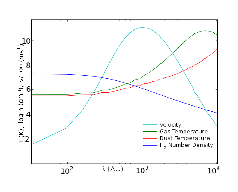
\includegraphics[width=84mm]{Figures/model/L1544model_used_legend_small.eps}
 \label{fig:l1544_model}
 \caption{Model of the pre-stellar core L1544 used as the envelope of the young protoplanetary disc in the hybrid model. Showing temperature (red) and dust (green) temperature in kelvin, log number density (blue) in cm$^{-3}$ and inward velocity$\times$100 (cyan) in m$\,$s$^{-1}$. Adapted from Keto \& Caselli (2010) and Keto et al. (2012, in preparation).}
\end{figure}


\begin{figure*}
 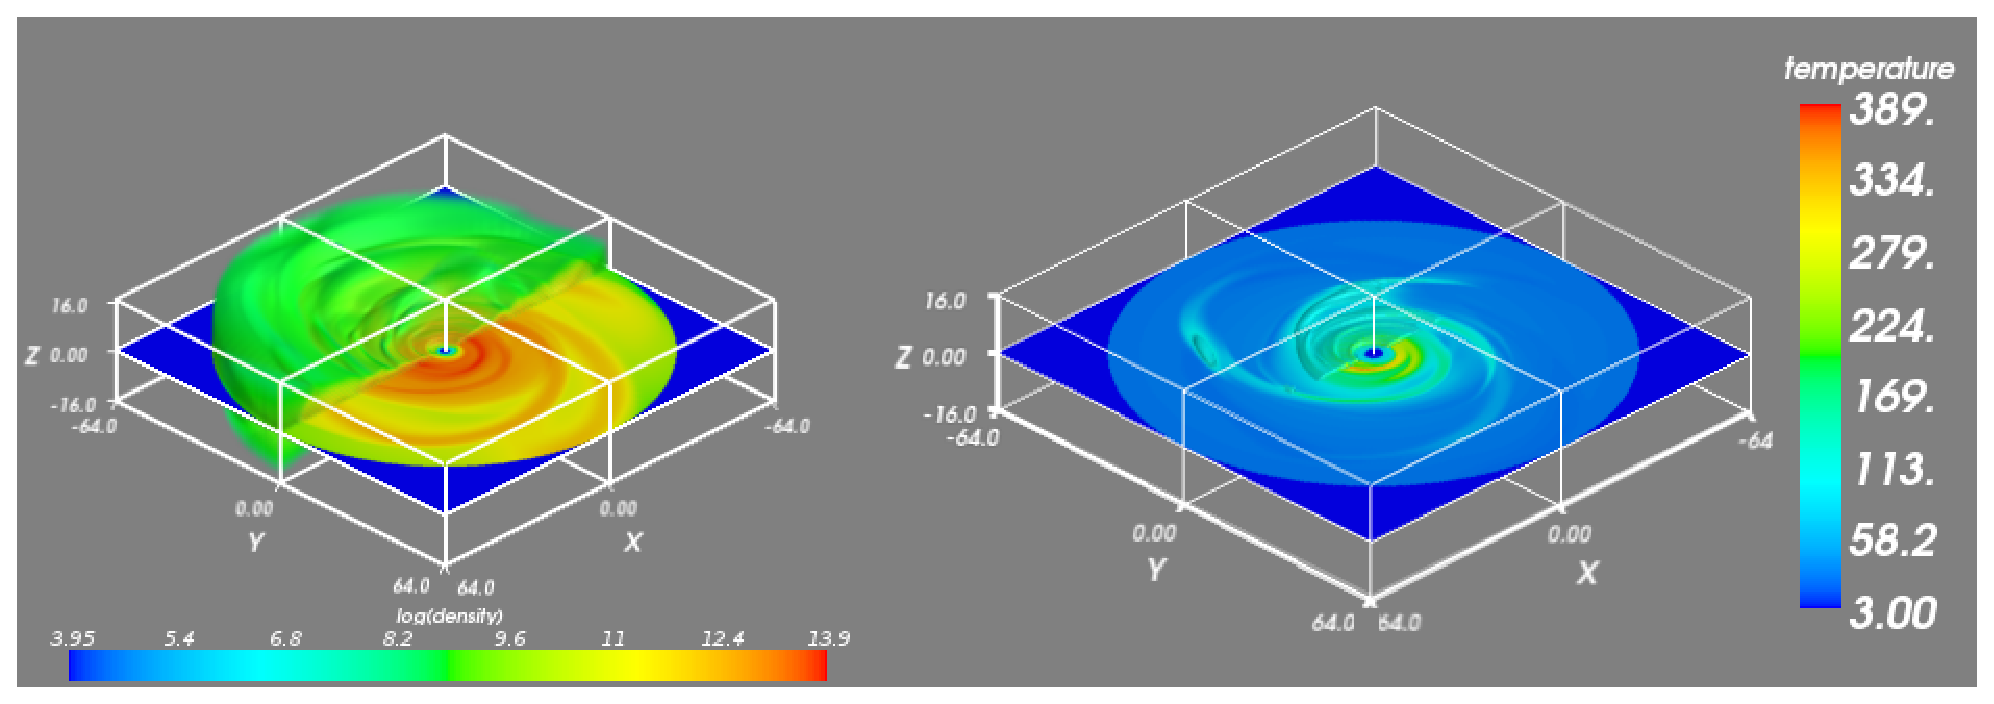
\includegraphics[width=168mm]{Figures/model/rhoT2.eps}
 \label{rhoT} 
 \caption{{\bf Left:} A 3D plot of log number density (cm$^{-3}$) showing the spiral structure in the xy plane and scale height of the disc. {\bf Right:} The 3D temperature structure of the disc; regions cooler than 40 degrees are not shown in 3D, demonstrating the narrow central region containing hot material.}
\end{figure*}

\begin{figure*}
 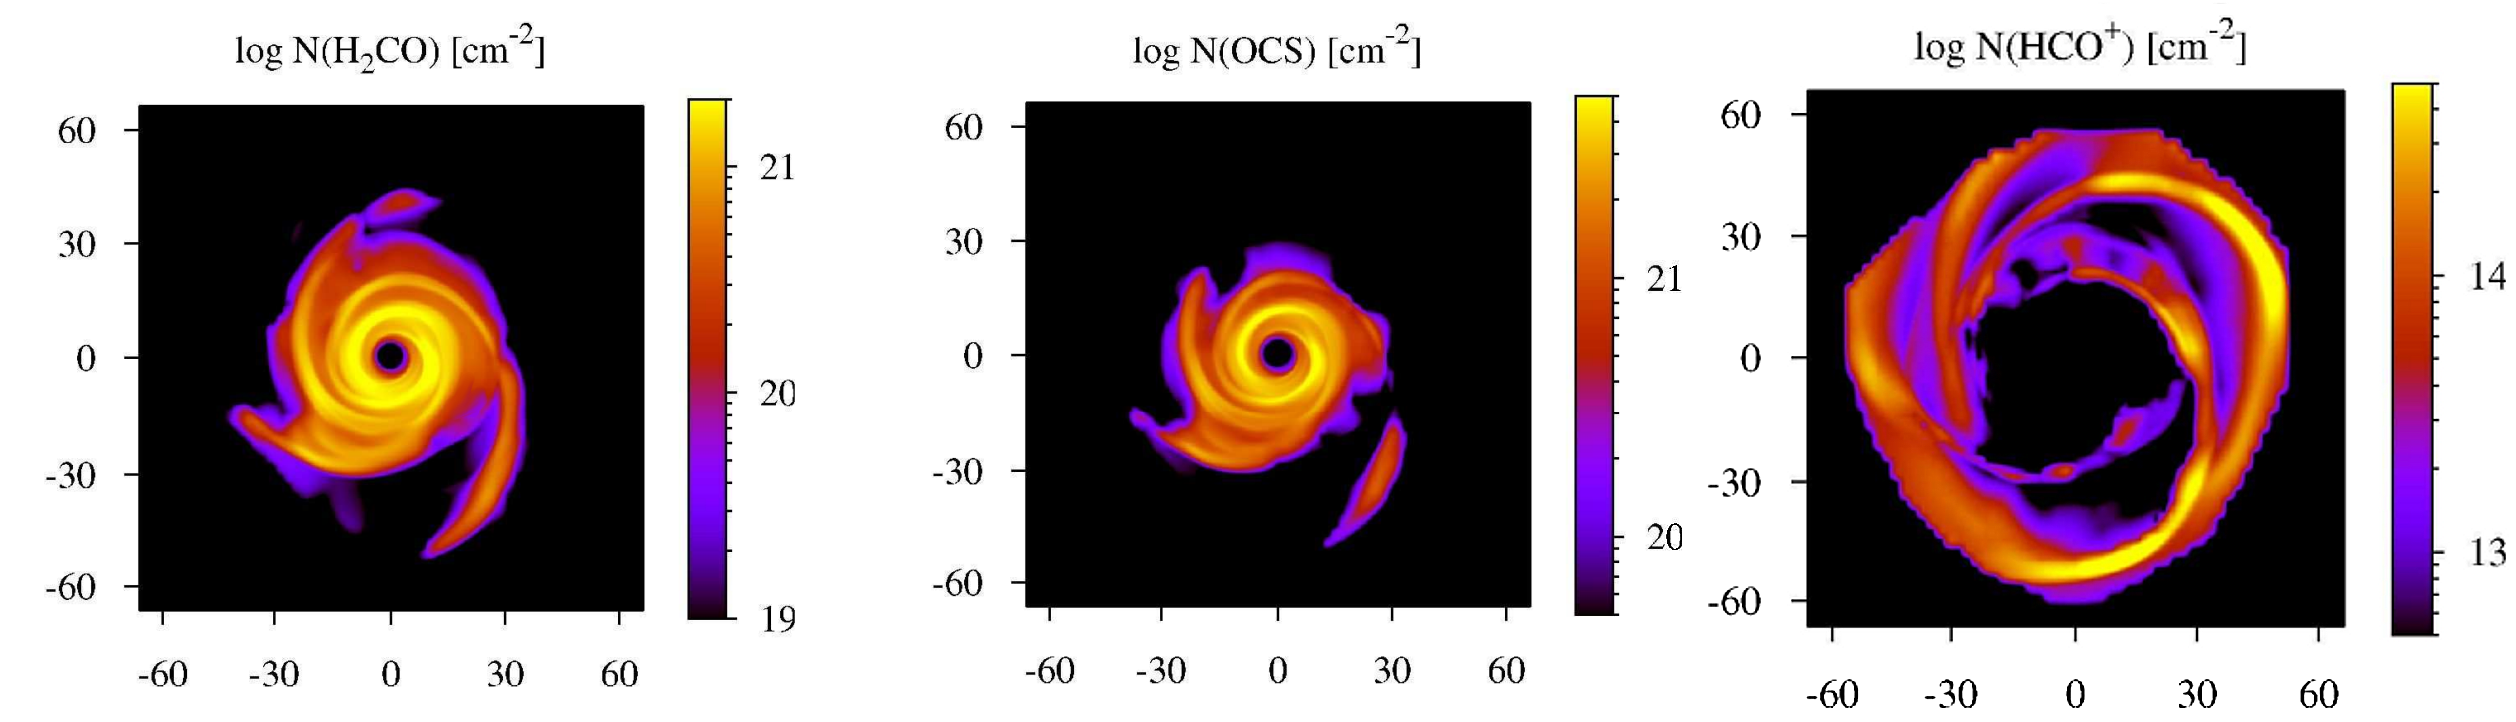
\includegraphics[width=168mm]{Figures/model/columnDensities2.eps}
 \label{Chemistry} 
 \caption{Column densities of OCS, H$_2$CO and HCO$^+$ used in the disc model. Figure adapted from Ilee at al. (2011) [SHOULD WE ALSO ADD C18O COLUMN DENSITY AS WE WANT TO DISCUSS THAT LATER ?? ]}
\end{figure*}

\begin{figure}
 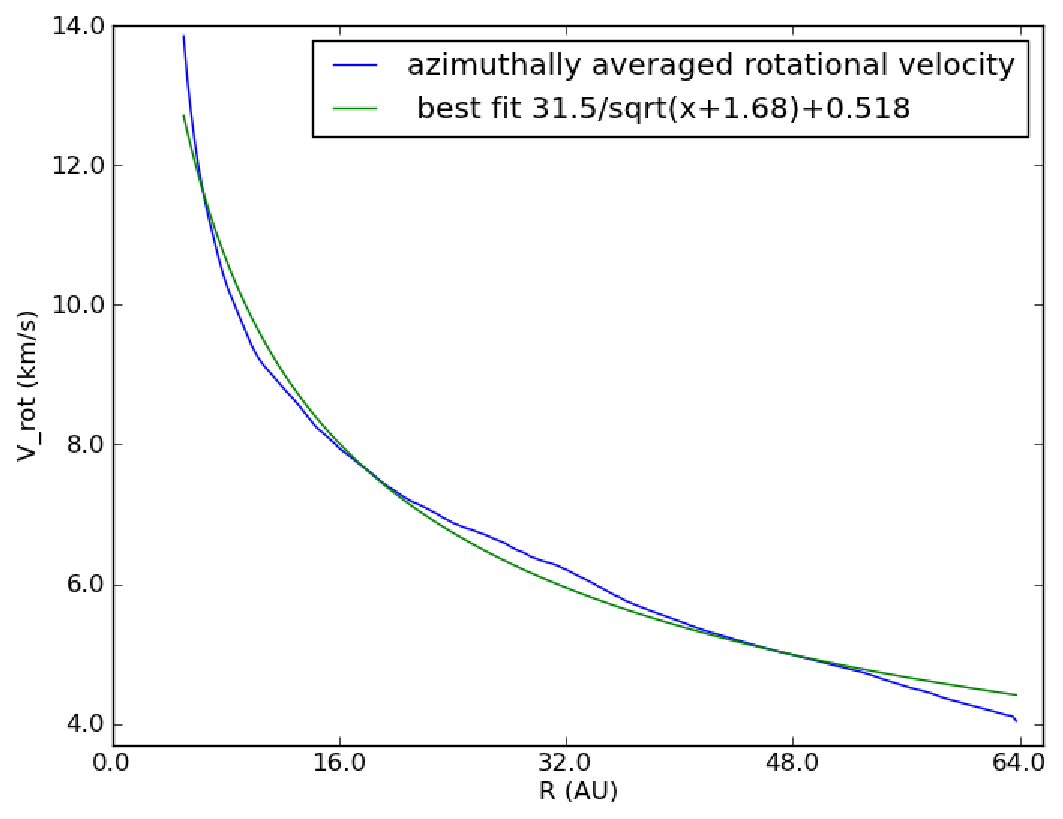
\includegraphics[width=84mm]{Figures/model/rotational_velocities.eps}
 \label{velocity}
 \caption{Azimuthaly averaged rotational velocity in the disc mid-plane with best fit curve}
\end{figure}


%-describe the physical structure of the disc (density and temperature) -- one figure showing the physical structure and the kinematics (2-panels figure)
The pre-stellar core structure is maintained down to a radius of 80\,AU, within which the young protoplanetary disc has been plugged in. The disc structure is derived by the hydrodynamic model of Boley(2007) and Boley (2009). The particular model considered here (as well as in Ilee et al. 2011) is a 0.39$\,\rm{M}_\odot$ self-gravitating disc featuring prominent spiral arms. H$_2$ number densities in the disc range from 10$^{4}$-10$^{13}\,\rm{cm}^{-3}$, and temperatures range from 30-400 K (figure \ref{rhoT}). The dust and gas temperatures in the disc are assumed to be in equilibrium. The model is sampled over a regular grid of size 256$\times$256$\times$64 with spatial resolution of 0.5$\,$au in x, y and z. The gas/dust mass ratio was assumed to be 1/100 throughout both sections model and the opacities were given by the model of dust grains with thick icy mantles and 10$^6\,$yr coagulation from Ossenkopf and Henning (1994). The gas number density and temperature structure are displayed in Fig. XX. \newline

%The majority of the mass lies in the mid-plane of the disc. For the models using a smoothed disc the same physical and chemical model is used but with the temperature, density and abundance averaged in $\phi$. The gas/dust mass ratio was assumed to be 1/100 throughout both sections model and the opacities were given by the model of dust grains with thick icy mantles and 10$^6\,$yr coagulation from Ossenkopf and Henning (1994)\newline

%-describe the chemistry  - refer to Ilee et al. which have been taken as input to the rad transfer (RT) code
Chemical abundances in the disc were taken from Ilee et. al (2011) which followed the changes of chemical abundances of trace particles moving through the disc as it evolved. The abundances of 125 species related by 1334 reactions were followed through the time evolution of the disc. These abundances were interpolated onto a 51$^3$ grid covering the disc with cells of size 2.2$\times$2.2$\times$0.22$\,$au.  From Ilee et al. (2011) we selected the three species which appear to trace different regions of the disc : the inner 30\,AU (OCS), the inner 60\,AU (H$_2$CO) and the region between $\simeq$20 and 60\,AU (HCO$^+$) and one which traces the entirety of the disc (C$^{18}$O). As explained by Ilee et al. (2011),  H$_2$CO and OCS mostly probe the central warm regions, where icy mantles evaporate, whereas HCO$^+$ preferentially traces the outer spiral pattern as in the central region it is destroyed by water molecules. The simple chemistry in the KC2010 model, adopted here as the envelope of the protoplanetary disc, does not provide detailed abundances of molecular species (besides CO and H$_2$O, see also Caselli et al. 2012). As discussed in the result section (Sec.\,\ref{sec:model_results}), rough guesses have been made based on values measured toward similar objects. 


\subsection{The radiative transfer code} \label{subsec:radiative_transfer_code}
%-describe the RT used (LIME) 
%-describe the RT used (LIME) 
The radiative transfer program used, LIME (Brinch \&Hogerheijde 2010), calculates line intensities based on a weighted sample of randomly chosen points in a continuous 3D model. The method of selecting these points is given in the grid-construction section. At each of these points, the density of the main collision partner (H$_2$), gas and dust temperatures, velocity, molecular abundances and turbulent velocity are taken from the model. These points are then smoothed by Lloyds algorithm (Lloyd 1982) in order to minimise the variation in distance between points whilst keeping the same underlying distribution. These points are then connected by Delaunay triangulation \footnote{In three dimensions this means that if four points are connected into a tetrahedron, the sphere circumscribing these four points contains no other points. It can be shown that this connection is unique for a given set of points.} and it is down these paths that photon propagation is restricted (figures \ref{grid}). The level populations of the selected molecules are calculated at each of these points from collisional and radiative (de)excitation and the local radiation field is calculated. This is repeated 20 times with the populations of each level converging towards a single value. This number of iterations is sufficient for the signal to noise ratio of the level populations (as defined in Brinch \&Hogerheijde 2010) to exceed 1000 in 99\% of the points, ensuring that the simulation has converged on a stable level population. \newline
After 20 iterations of updating the level populations the model is ray-traced in order to produce synthetic brightness maps. In order to minimise the artifacts in the output images, resulting from the grid construction, the average of ten separate runs was taken (figure \ref{averages}).


%\begin{figure}
% 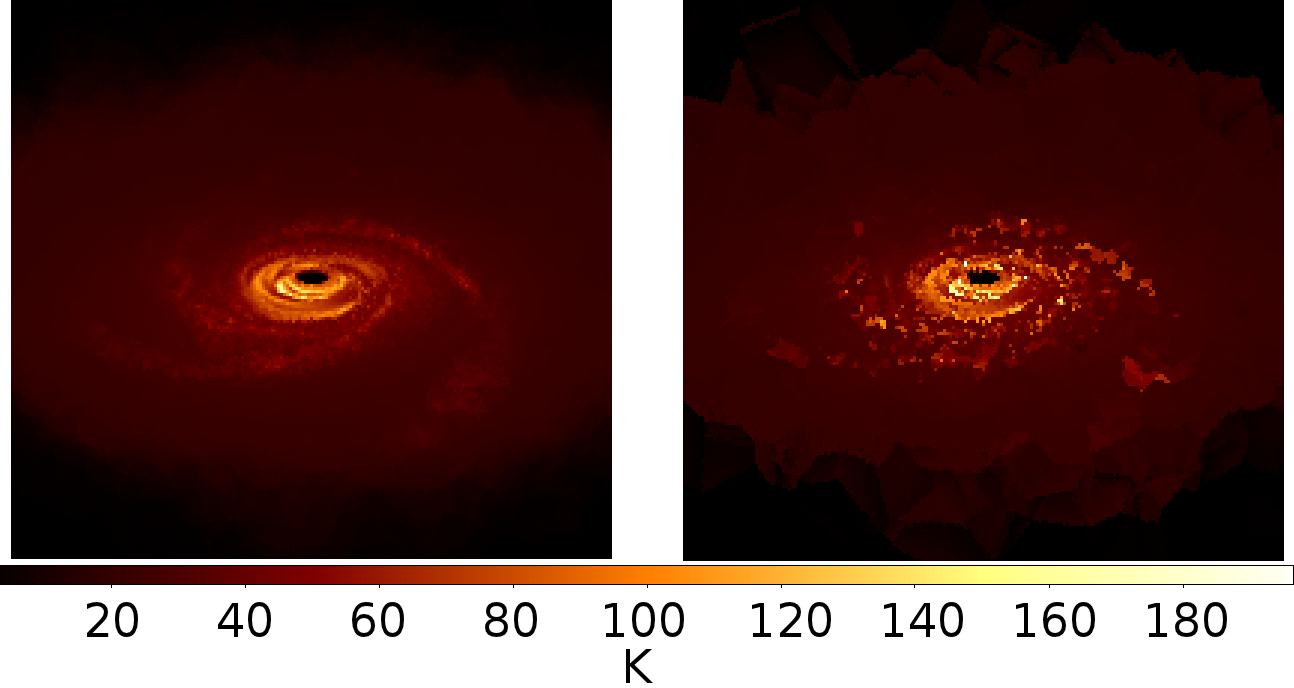
\includegraphics[width=84mm]{Figures/sim/average_comparison.eps}
% \label{averages}
% \caption{A plot showing the difference between a single LIME continuum image at 300$\,$GHz (right) and the average of ten such images from different runs of the same model in LIME (left).}
%\end{figure}


\begin{figure}
 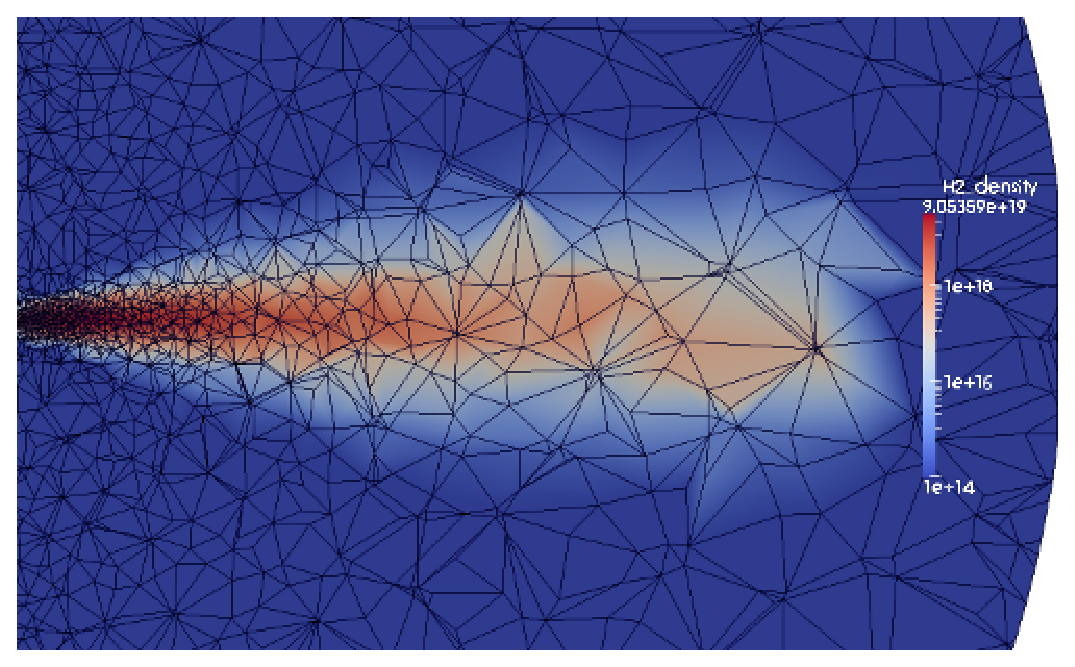
\includegraphics[width=84mm]{Figures/model/Lime_grid3.eps}
 \label{grid}
 \caption{A plot of the points selected by the griding process and the paths down which photons can propagate overlaid on a smoothed density model. The points are more concentrated at small radii and in the densest regions.}
\end{figure}

\begin{figure}
 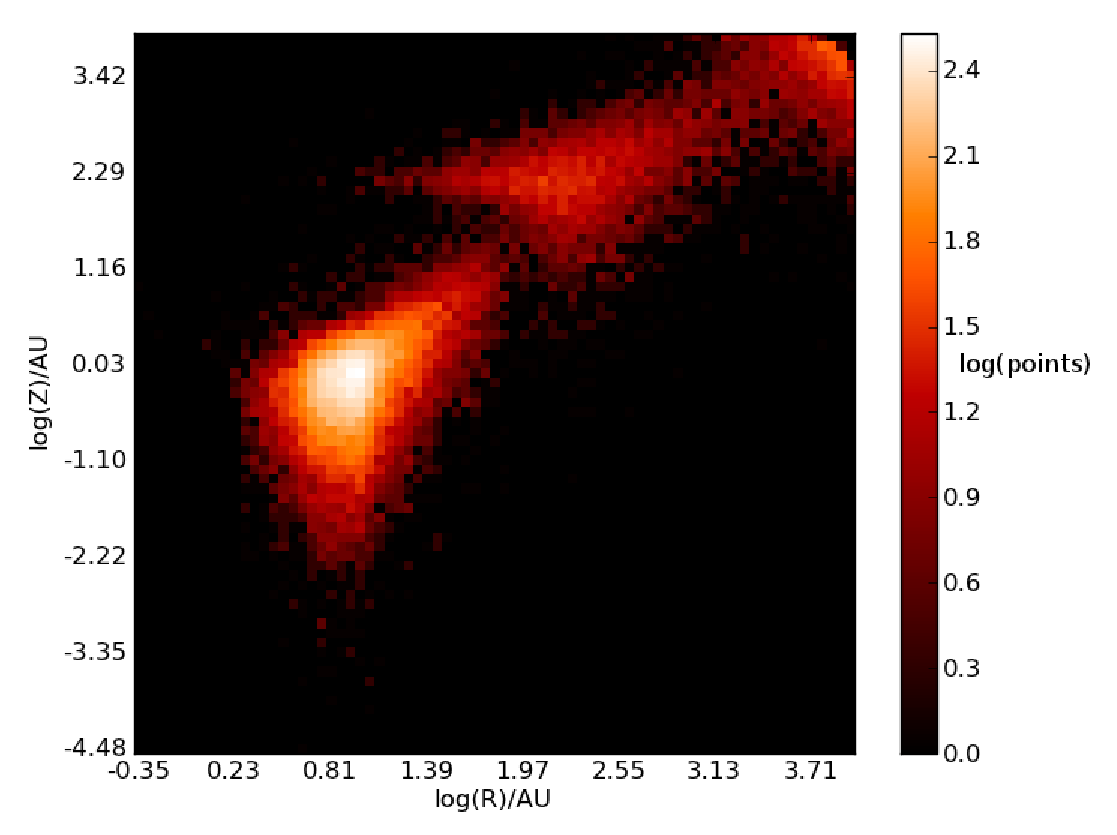
\includegraphics[width=84mm]{Figures/model/lime_points_rz_histo2.eps}
 \label{points}
 \caption{A 2D histogram of the point distribution throughout the model. The disc and envelope can be seen as two separate entities which have to be sampled using different point distributions}
\end{figure}

\section{Model Results} \label{sec:model_results}

Simulations are limited to molecules for which we have abundances in both the disc and envelope, and also have calculated Einstein and collisional coefficients. The Molecular data used is from the lamda database (reference? http://home.strw.leidenuniv.nl/$\sim$moldata/). Lines for the molecules which satisfy these conditions were simulated with LIME for frequencies between 50$\sim$500$\,$GHz, with a focus on lines which could be observed in ALMA band 7 and molecules which are not typically seen in outflows. The results presented in this section represent those lines which show detectable emission/absorption which can be used to trace either spiral structure or rotation.\newline

Transitions focused upon are CO 3-2 (and isotopologues) at 345.8GHz with an upper energy level of 33.2K, HCO+ 1-0 at 89.2GHZ and 4.3K, OCS 28-27 at 340.4GHz and 237.0K and H2CO $4_{04}$-3$_{03}$ at 290.6GHz and 34.9K {\bf maybe worth including a higher frequency line as well? CS at ~650GHz?}. Other molecules simulated but not shown include HCN, HNC, HNO, HCS$^+$ and CS.\newline

For the purpose of simulating observations the model was placed at roughly the distance of nearby low-mass star forming regions (100$\,$pc) and is inclined at 30$^\circ$ to edge on. From these observations integrated intensity, intensity weighted velocity and position velocity diagrams through the centre of the model were created.
The simulations done are focused upon frequencies within ALMA band 7, selected to give the best trade off between resolution and sensitivity for early ALMA science.
(Note the moment 1 and 0 maps were created by integrating between -12.5 to -0.5 km$\,$s$^{-1}$ and +0.5 to +12.5 km$\,$s$^{-1}$ to avoid being dominated by the contribution from the envelope, this can be seen in some PV diagrams as the strong absorption feature at all positions around zero velocity, moment 1 maps are shown with a cut-off of 1/100 of the peak emission/absorption value)\newline

\begin{figure}
 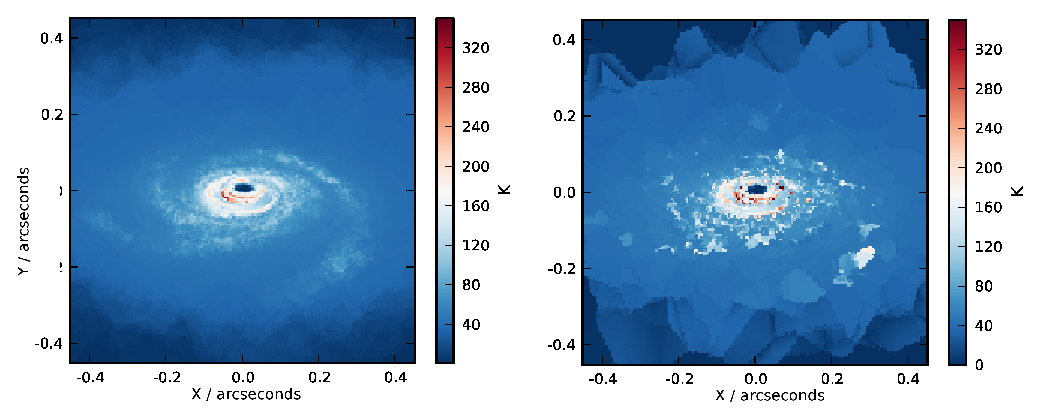
\includegraphics[width=84mm]{Figures/sim/continuum.eps}
 \label{points}
 \caption{A 300$\,$GHz continuum image of the model, created from the average of ten LIME runs.}
\end{figure}

\begin{figure*}
 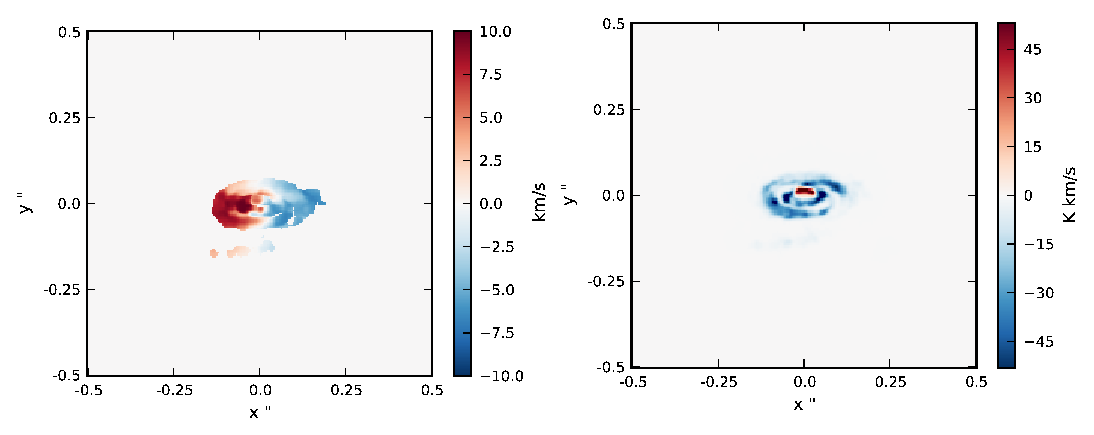
\includegraphics[width=168mm]{Figures/sim/imageOCS_28-27_30deg_composite_all.eps}
 \label{OCS_all}
 \caption{OCS 28-27 {\bf Left:} Continuum subtracted integrated intensity map showing clearly differentiated spiral structure in the inner regions of the disc, {\bf Right:} Intensity weighted velocity map}
\end{figure*}


%\begin{figure}
% 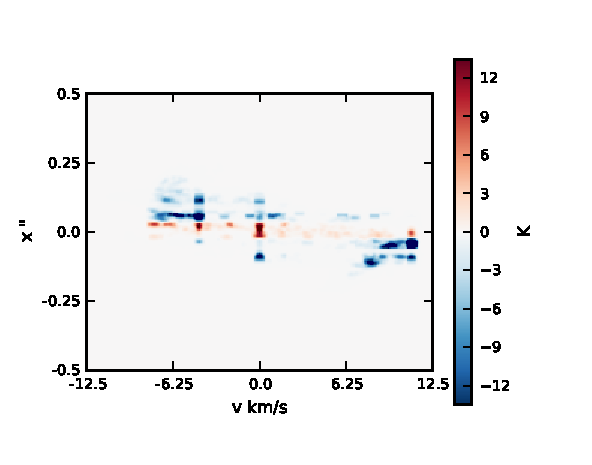
\includegraphics[width=84mm]{Figures/sim/imageOCS_28-27_30deg_composite_PV_centre.eps}
% \caption{OCS 28-27 position-velocity diagram through centre}
%\end{figure}


OCS traces only the innermost region of the disc and can be used to examine the central regions. As OCS is not seen in outflows it can be used to view rotation of the central part of the disc without risk of contamination. As the excitation energy for the high J transitions of OCS is much higher than the other lines under consideration it is only excited in the hottest densest regions. As a result of this the spiral structure is clearer in OCS than in most transitions, with the low density regions between spiral arms showing no emission or absorption(see figure \ref{ocs_all}). The majority of the OCS is visible in absorption against the bright continuum emission from the disc midplane. The exception to this in the centre of the disc and is an effect of the inclination angle, whereby the line of sight passes through gas above the midplane and then through the hole in the centre of the disc. 

%\begin{figure}
% 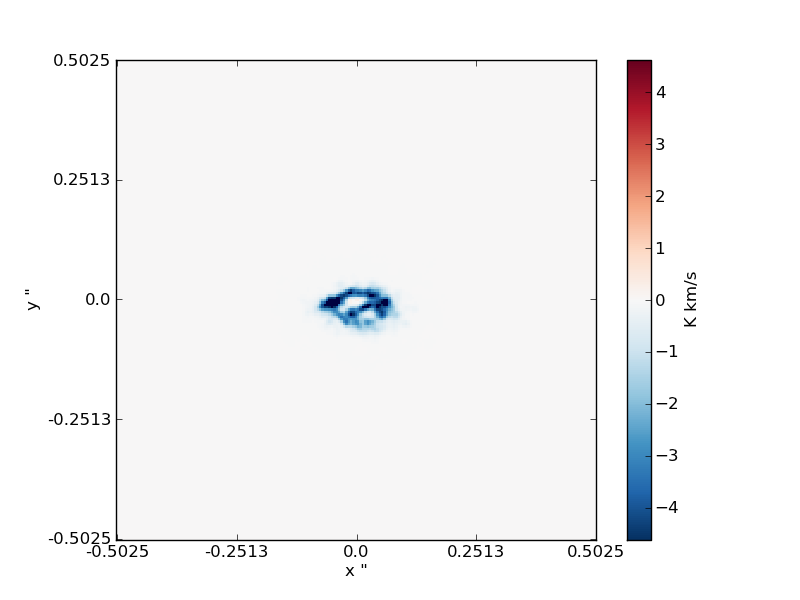
\includegraphics[width=84mm]{Figures/sim/imagesmoothedOCS_28-27_30deg_contSub.png}
% \label{smoothOCS_mom0}
% \caption{SmoothedOCS 28-27 Continuum subtracted mom0}
%\end{figure}
 
%\begin{figure}
% 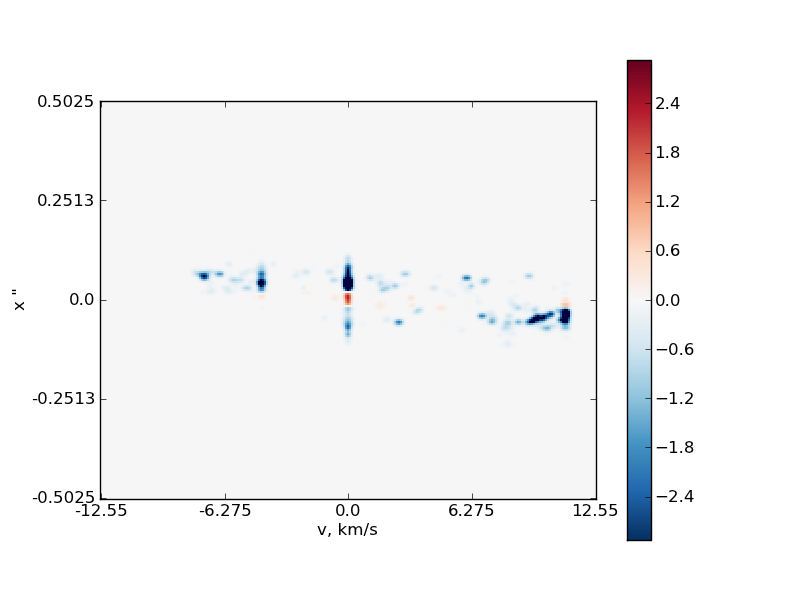
\includegraphics[width=84mm]{Figures/sim/imagesmoothedOCS_28-27_30deg_PV_centre.png}
%
% \caption{SmoothedOCS 28-27 PV through centre}
%\end{figure}


\begin{figure*}
 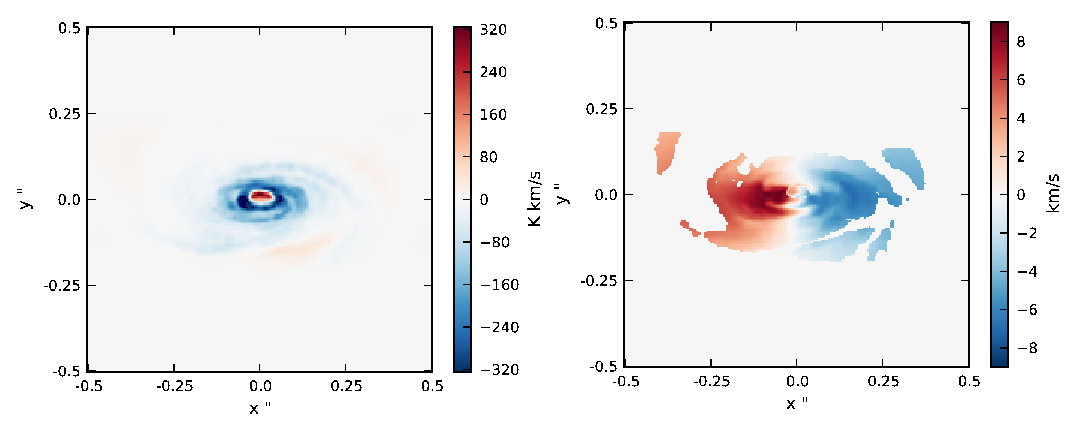
\includegraphics[width=168mm]{Figures/sim/imageH2CO_4-0-4--3-0-3_30deg_composite_all.eps}
 \label{h2co_all}
 \caption{H$_2$CO 4$_{0\,4}$ - 3$_{\,0\,3}$ {\bf Left:} Continuum subtracted integrated intensity map, {\bf Right:} Intensity weighted velocity map}
\end{figure*}

%\begin{figure}
% 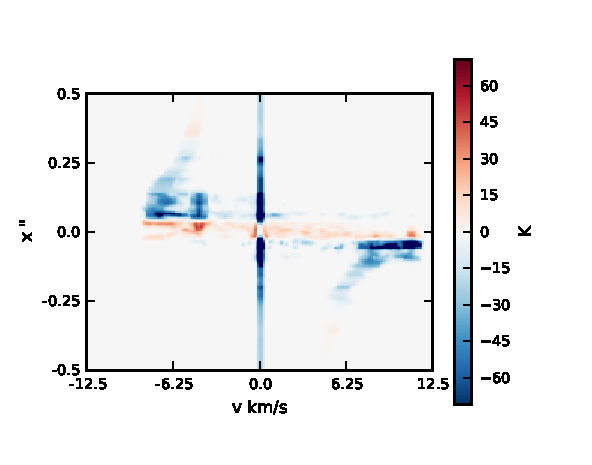
\includegraphics[width=84mm]{Figures/sim/imageH2CO_4-0-4--3-0-3_30deg_composite_PV_centre.eps}
% \caption{H$_2$CO 4$_{0\,4}$ - 3$_{\,0\,3}$ PV through centre}
%\end{figure}

The abundance H$_2$CO molecule is fairly typical of the molecules simulated in Ilee (2011) in that it traces the spiral structure roughly the inner 2/3$^{rd}s$ of the disc. The spiral structure of the disc can be seen clearly in the integrated intensity map and its rotation of detected out to larger radii than is possible with the OCS and is more visible between spiral arms but is otherwise simimlar in morphology.

\begin{figure*}
 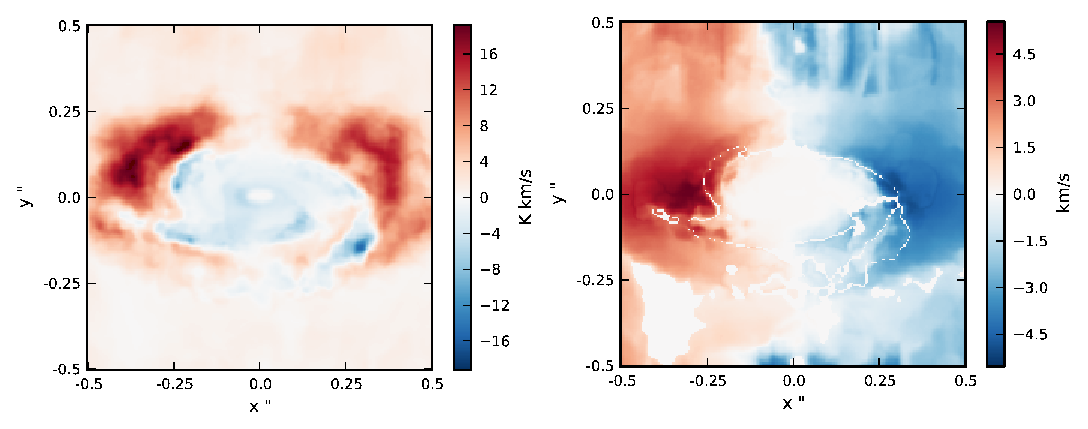
\includegraphics[width=168mm]{Figures/sim/imageHCOp_1-0_30deg_composite_all.eps}
 \label{h2co_all}
 \caption{HCO$^+$ 1-0 {\bf Left:} Continuum subtracted integrated intensity map, {\bf Right:} Intensity weighted velocity map}
\end{figure*}

%\begin{figure}
% 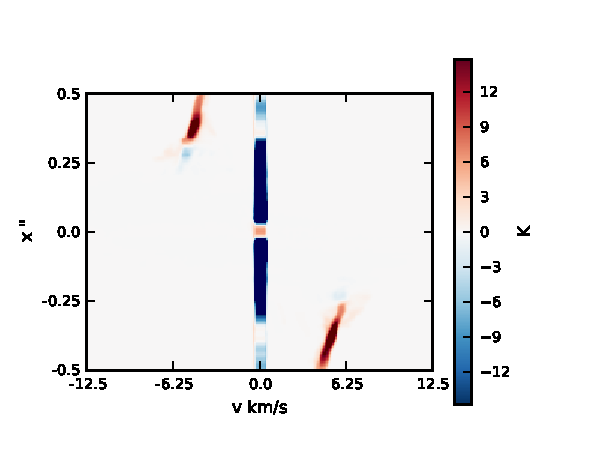
\includegraphics[width=84mm]{Figures/sim/imageHCOp_1-0_30deg_composite_PV_centre.eps}
% \caption{HCO$^+$ 1-0 pv through centre, with the rotation curve from figure \ref{velocity} for comparison}
%\end{figure}

%\begin{figure}
% 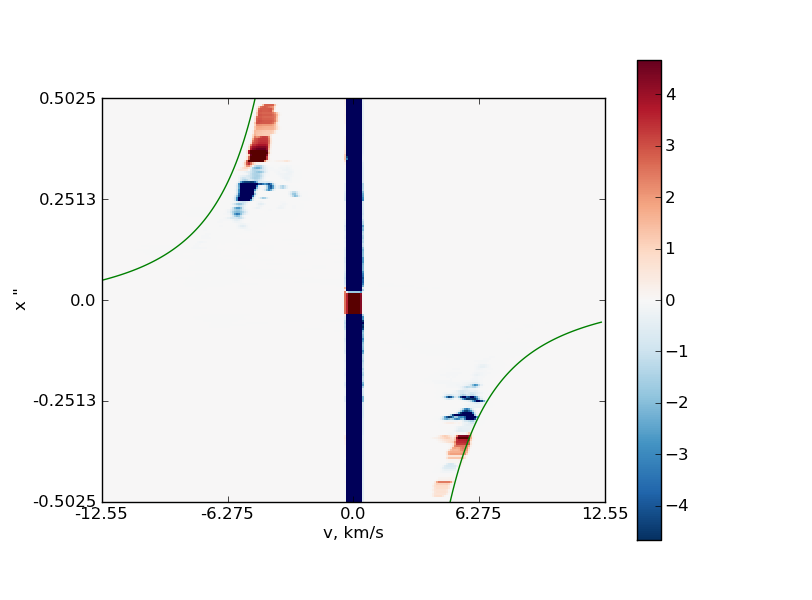
\includegraphics[width=84mm]{Figures/sim/imageHCOp_3-2_30deg_PV_centre_2.png}
% \label{hcop_pv}
% \caption{HCO$^+$ 3-2 PV through centre with rotation curve from figure \ref{velocity} *** should the velocities in this be reduced by cos(30) as we're not in the plane of rotation? ***}
%\end{figure}

Some molecules such as HCO$^+$ trace only the outer regions of the disc (Ilee 2011) and so can be used to look at the extended velocity and physical structure. In these colder less dense regions we see the molecular lines in emission rather than absorption. Figure \ref{hcop_pv} shows the rotation curve of the model as shown in figure \ref{velocity} against the HCO$^+$ J=1-0 line emission. It is clear that from observations such as these the rotation curve of a disc could be reconstructed.\newline

In all the simulations except HCO$^+$ we see molecular lines in absorption throughout the majority of the disc and in some cases a small amount of emission towards the centre. Molecular lines throughout the plane of the disc show up in absorption against the continuum emission of the shock heated, dense mid-plane. 





\section{ALMA Predictions} \label{sec:alma_predictions}

In order to make predictions on the observability of the synthetic brightness maps created by LIME, CASA (common astronomy software applications) was used to simulate observing these with the completed ALMA in its most extended comfiguration for a total time of four hours.

\begin{figure}
 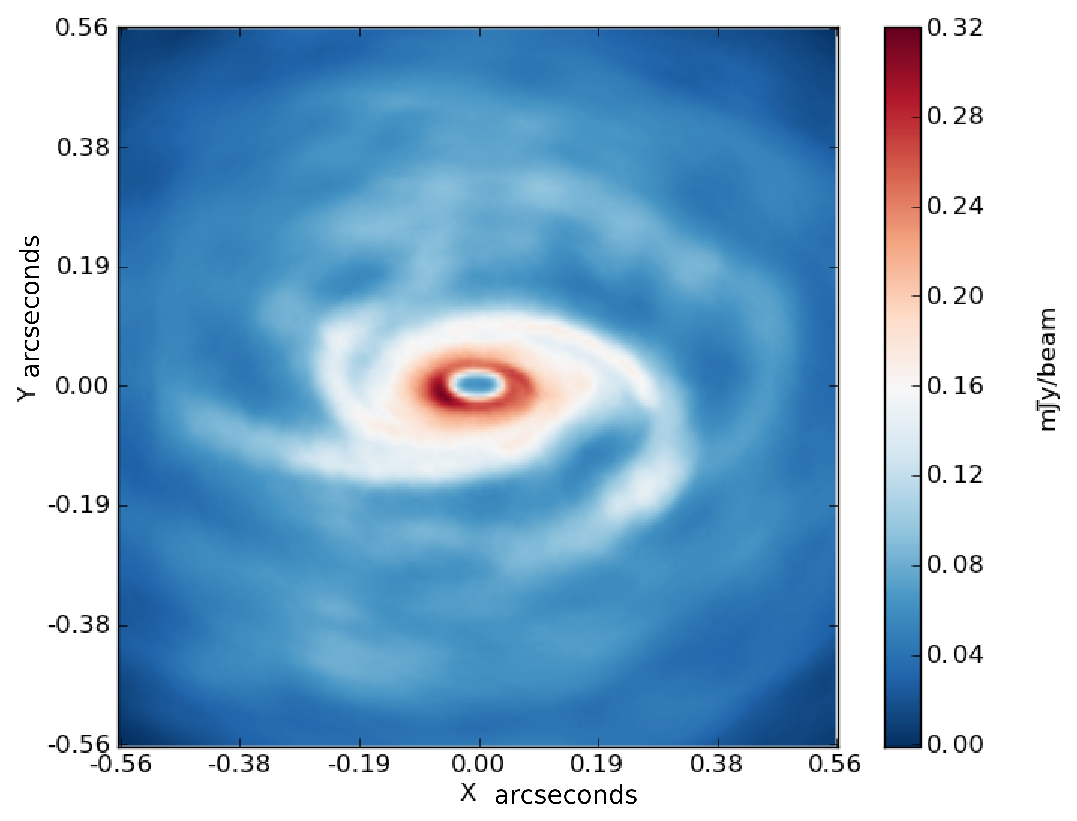
\includegraphics[width=84mm]{Figures/sim/casa_cont_337GHz.eps}

 \caption{Continuum emission at 337GHz simulated for ALMA most extended configuration}
\end{figure}

\begin{figure}
 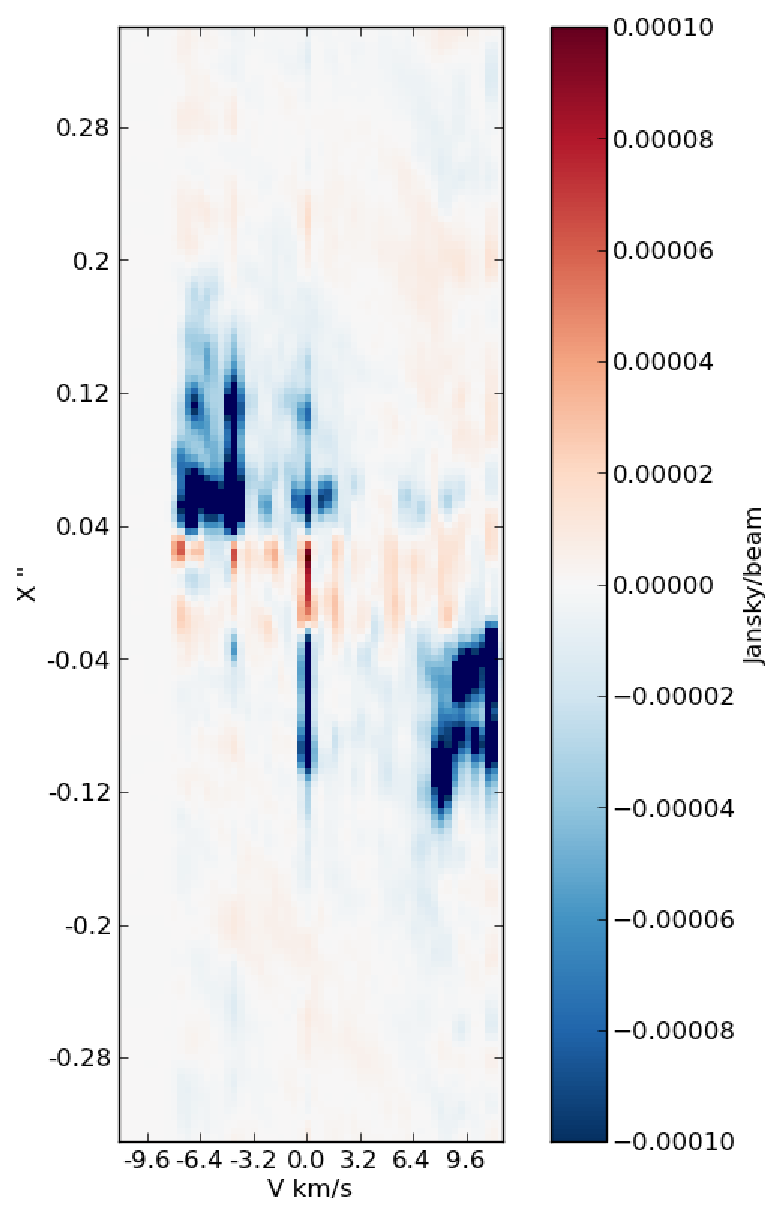
\includegraphics[width=54mm]{Figures/sim/casa_imageOCS_28-27_30deg_composite_ALMAwidth_big_dirty_PV_centre.eps}

 \caption{OCS 28-29 pv diagram simulated for ALMA most extended configuration}
\end{figure}


\begin{figure}
 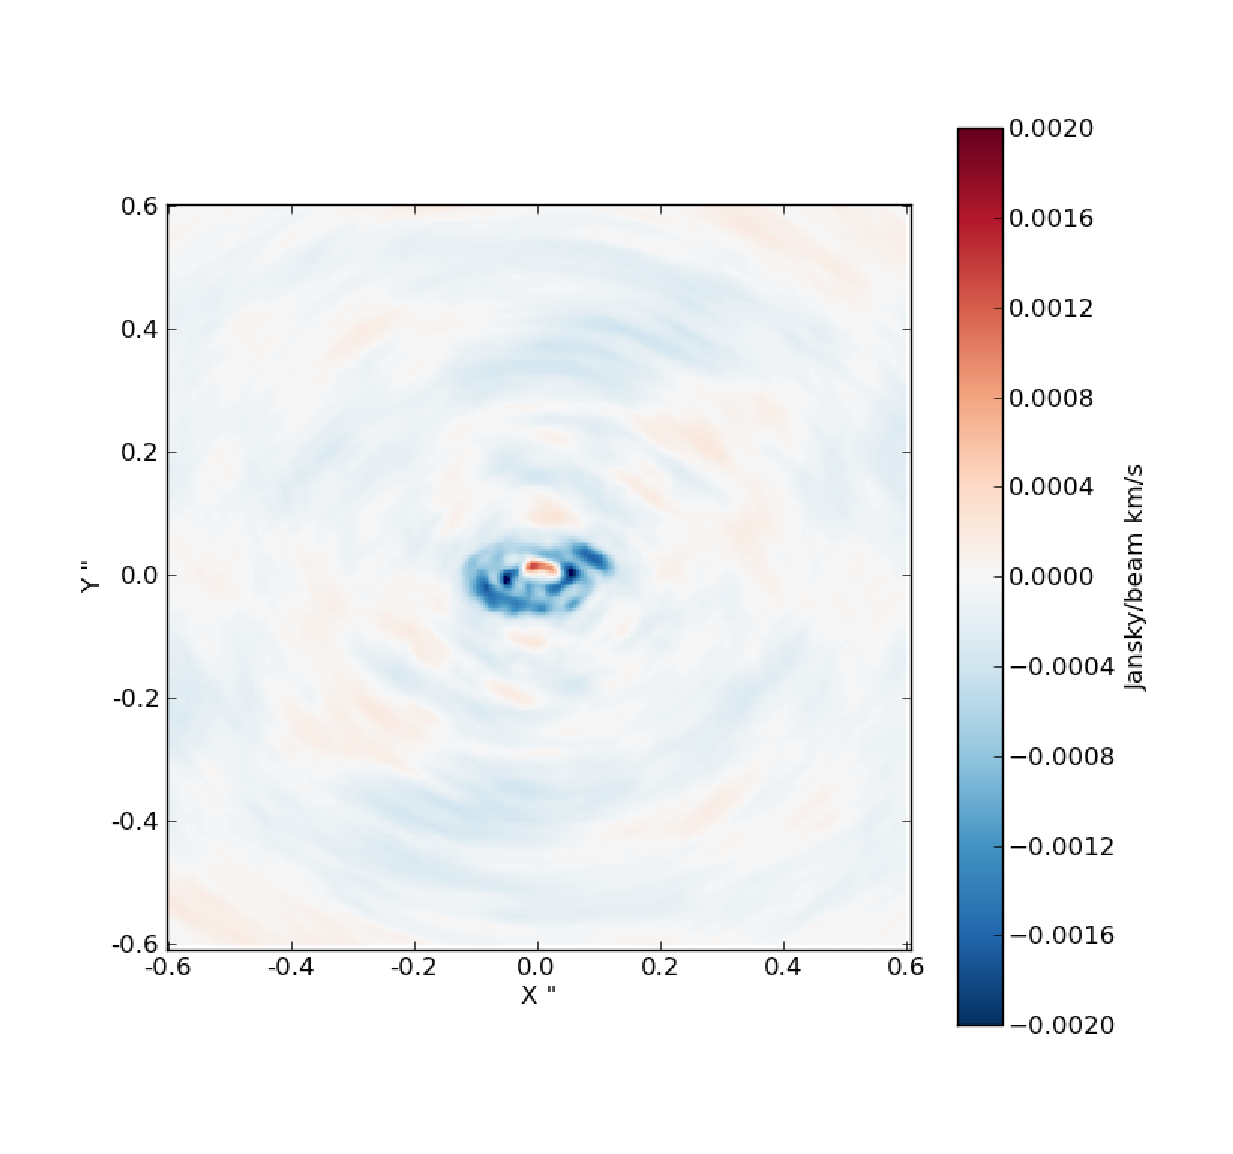
\includegraphics[width=84mm]{Figures/sim/casa_imageOCS_28-27_30deg_composite_ALMAwidth_big_dirty_contSub.eps}

 \caption{OCS 28-29 integrated intesity simulated for ALMA most extended configuration}
\end{figure}

\begin{figure}
 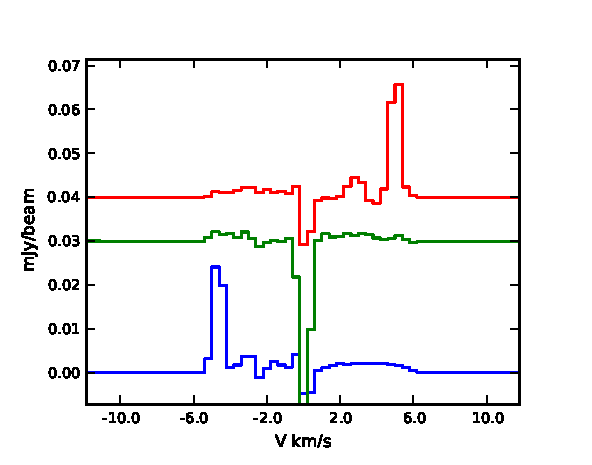
\includegraphics[width=84mm]{Figures/sim/casa_HCOp_spectra_40_AUsplit.eps}

 \caption{HCO$^+$ 1-0 30 deg spectra at Y=0, X=+40AU (bottom), 0AU (middle) and -40AU (Top)}
\end{figure}

\begin{figure}
 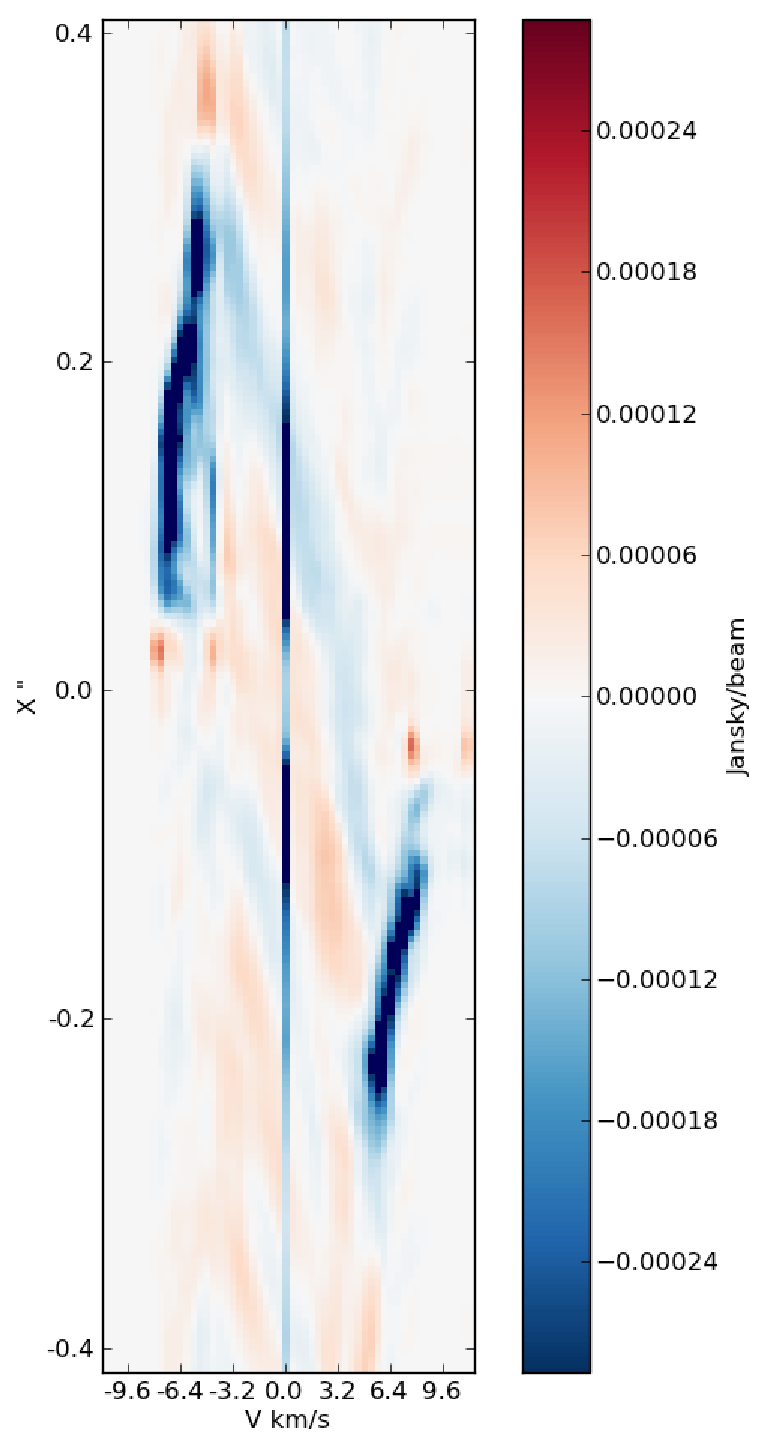
\includegraphics[width=54mm]{Figures/sim/casa_imageC17O_3-2_30deg_composite_ALMAwidth_dirty_PV_centre.eps}

 \caption{C$^{17}$O 3-2 30 deg PV through centre simulated for ALMA most extended configuration}
\end{figure}

\begin{figure}
 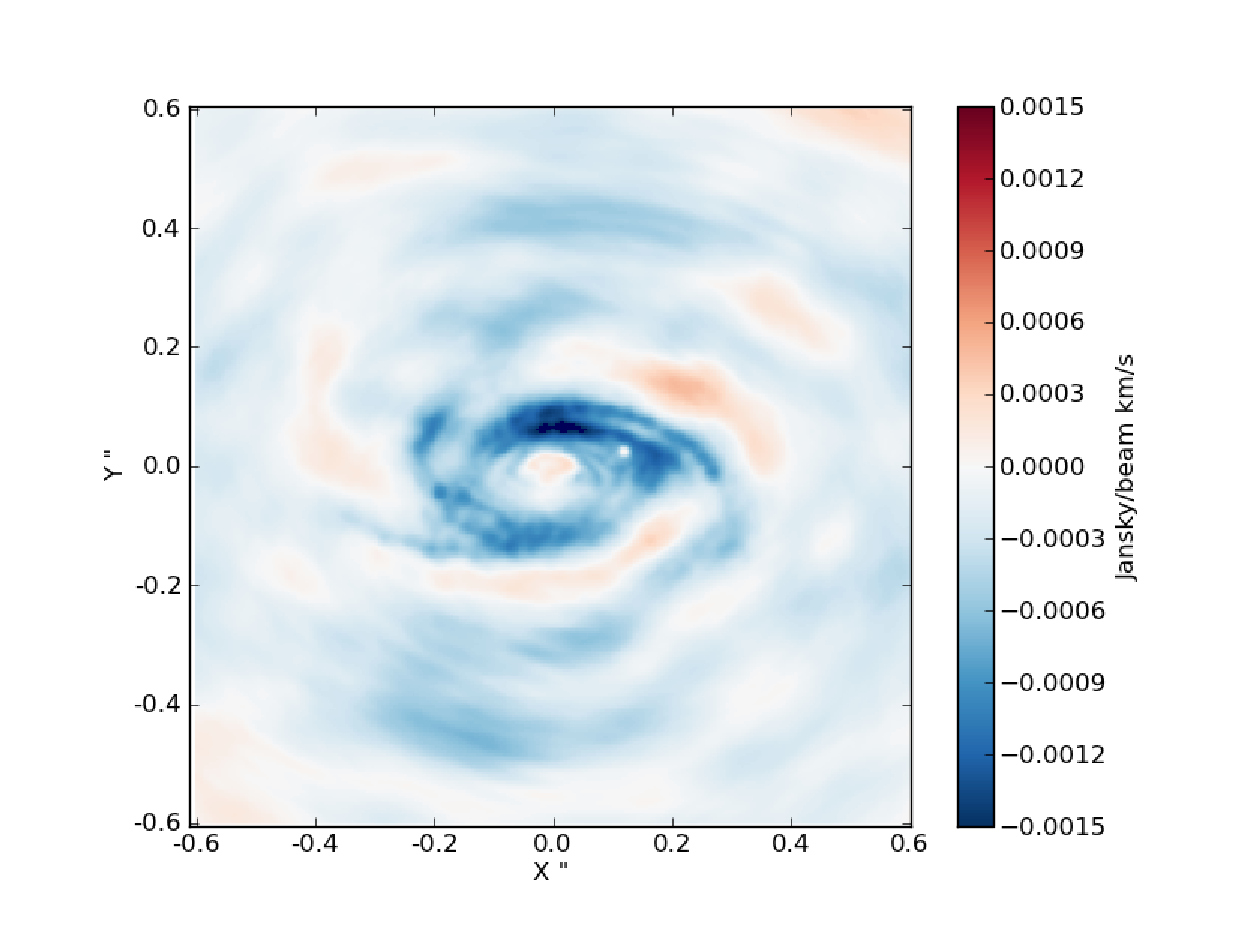
\includegraphics[width=84mm]{Figures/sim/casa_C17O_3-2_mom0.eps}

 \caption{C$^{17}$O 3-2 30 deg integrated intensity simulated for ALMA most extended configuration}
\end{figure}

\begin{figure}
 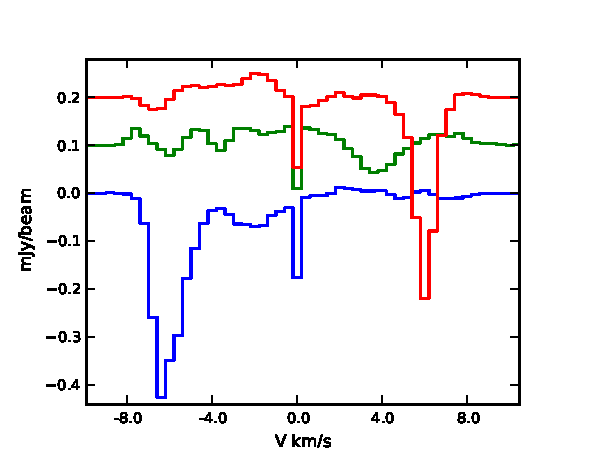
\includegraphics[width=84mm]{Figures/sim/casa_C17O_spectra_20AUsplit.eps}

 \caption{C$^{17}$O 1-0 30 deg spectra at Y=0, X=+20AU (bottom), 0AU (middle) and -20AU (Top)}
\end{figure}

\begin{figure}
 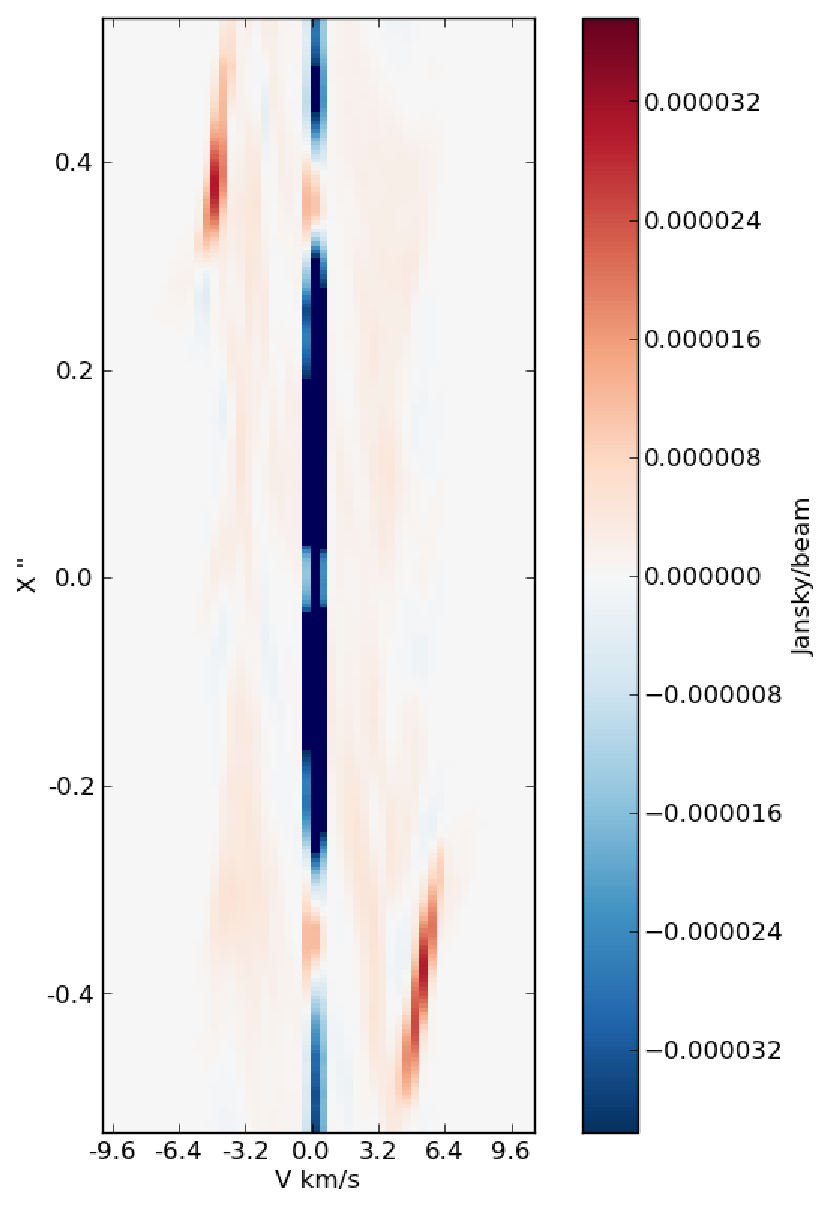
\includegraphics[width=63mm]{Figures/sim/casa_imageHCOp_1-0_30deg_composite_ALMAwidth_dirty_PV_centre.eps}

 \caption{HCO$^+$ 1-0 30 deg PV through centre simulated for ALMA most extended configuration}
\end{figure}

\begin{figure}
 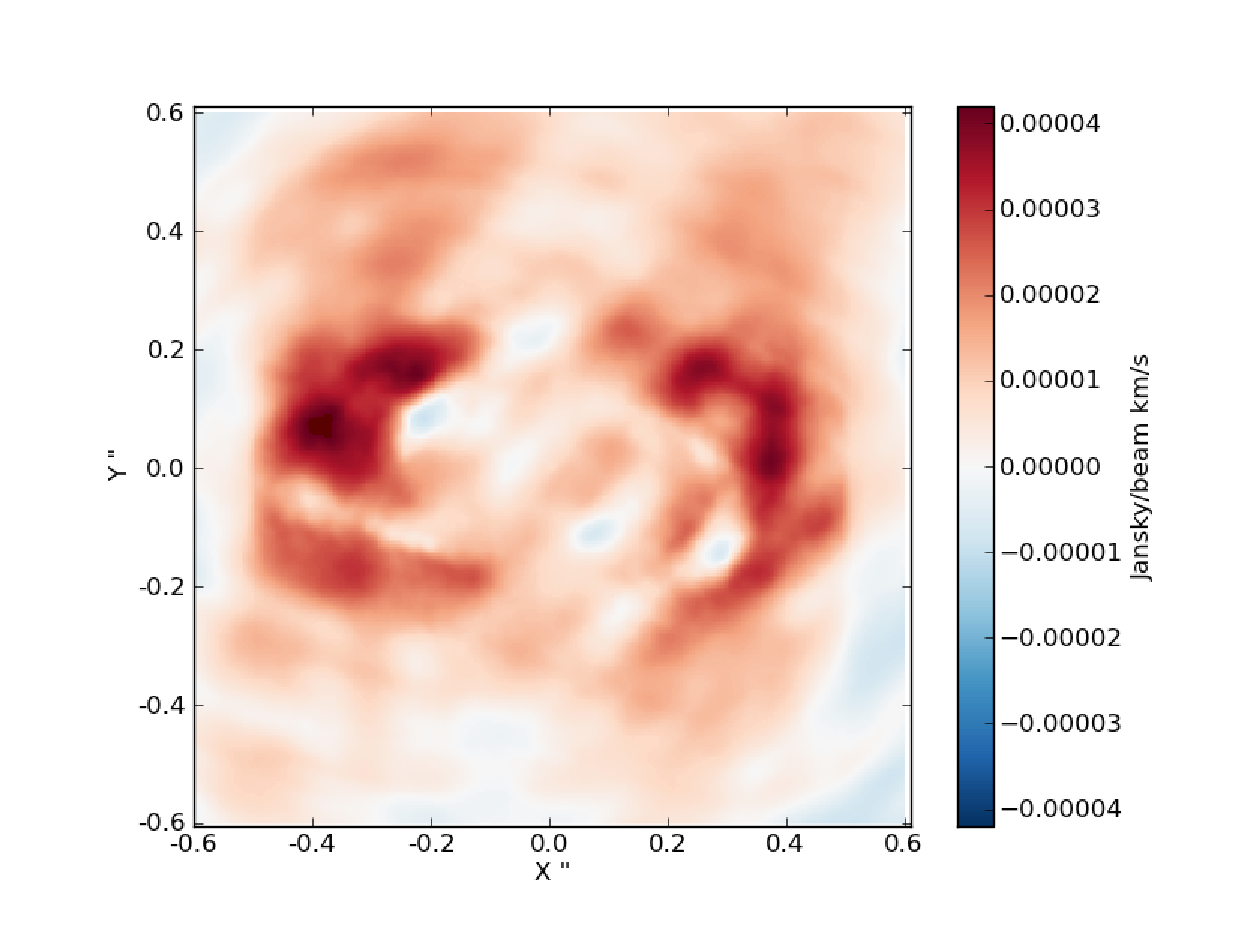
\includegraphics[width=84mm]{Figures/sim/casa_imageHCOp_1-0_30deg_composite_ALMAwidth_dirty_contSub.eps}

 \caption{HCO$^+$ 1-0 30 deg integrated intensity simulated for ALMA most extended configuration}
\end{figure}

\begin{figure}
 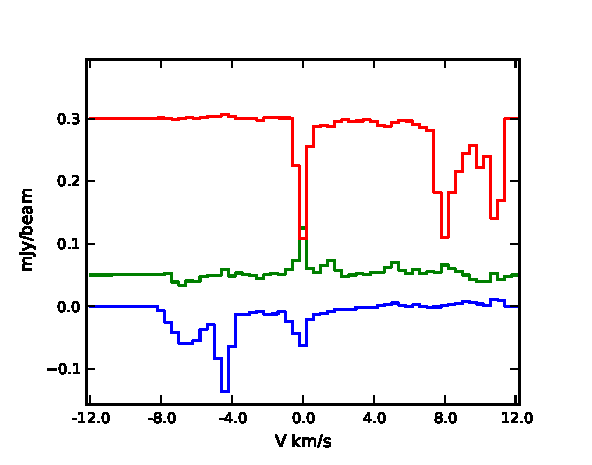
\includegraphics[width=84mm]{Figures/sim/casa_OCS_spectra_10AUsplit.eps}

 \caption{OCS 28-27 30 deg spectra at Y=0, X=+10AU (bottom), 0AU (middle) and -10AU (Top)}
\end{figure}

PV diagrams allow us to reconstruct the rotation of the disc. ALMA has enough resolution and sensitivity to see spiral structure clearly in continuum emission but also in CO isotopologues and marginally in OCS.


\section{Discussion and conclusions} \label{sec:discussion}

In this paper we have performed radiative transfer simulations of a hybrid model comprising a 0.4$\, M_\odot$ self gravitating disc with radius 64$\,AU$ showing spiral density waves, surrounded by an envelope simulated as a collapsing 10$\,M_\odot$ BE-sphere. CASA simulations show that at a distance of 100$\,$pc both spatial resolution of the spirals in such a disc and extraction of kinematic and temperature from molecular lines are possible in ALMA band 7. Our simulations show that many  molecular species are predominantly seen in absorption towards the centre of  self-gravitating protoplanetary discs. The quiescent nature of the envelope around such discs only obscures them within $\pm\,0.5 km\,s^{-1}$.\newline
One assumption made in this model is that the gas and dust are in thermal equilibrium.If they are not and the dust is significantly cooler than the gas then transitions may not show up in absorption.\newline
%The mass of the disc used (0.4$\,\rm{M}_\odot$) is on the high end for early discs (citations for estimate of early class 1 disc masses).\newline
In the model spirals shock heat the mid-plane layer and the colder more diffuse gas absorbs the continuum from it, this results in molecular lines being seen in absorbtion whenever lines of sight pass through the cold diffuse gas at larger heights on to the hot dense midplane of the disc. Rotation curves can be gathered from these observations even with spiral structure\newline
Outflows could contaminate measurements of rotation curves meaning that speices  which commonly trace outflows, such as CO and HCO$^+$ are not going to be good tracers of disc rotation. However speices such as OCS and C$^{18}$O which are not commonly seen in outflows (e.g. van der Tak et al. 2003, Stanke et al. 2007, Yildiz et al 2012, Ren et al. 2011)can be used to trace disc rotation.


\section*{Acknowledgements}

stuff here
\newpage

\appendix

\section{Grid Construction} \label{sec:gridding} 

In order to construct the grid, candidate points are randomly selected from the volume to be simulated. These candidates then have their density and molecular density compared against a reference point in order to decide if the point is to be used in the grid or not. Candidate grid points are selected at random in cylindrical co-ordinates, linearly spaced in z and $\phi$ and logarithmically spaced in r. For each point to be selected, a random number $\alpha$ is drawn from the semi-open set [0,$\,$1) as a threshold. After selection of random co-ordinates, the hydrogen density and molecular density at the candidate point (n and m, respectively) are compared against the densities of a reference point on the inner edge of the disc (n$_0$ and m$_0$). If $\alpha<\left( \frac{n}{n_0} \right)^{0.3}$ or $\alpha< \left( \frac{m}{m_0} \right)^{0.3}$ then the point is selected for use, otherwise another r, $\phi$, z co-ordinate is selected and this becomes the candidate point. The function comparing the candidate point to the reference point and the candidate point distribution were selected empirically to sample all the scales while ensuring that the majority of points are located in the inner disc where the density is higher. 20\% of these points are forced to be at radii greater than $\sqrt{R_{min}R_{max}}$ (where $R_{min}$ and $R_{max}$ are the inner and outer radius of the model) in order to stop too many of the selected points clustering in the high density disc and leaving the envelope under sampled. In addition to this method of selection, 5\% of the points are linearly distributed in x, y and z with no bias with regards to density or abundance. This provides a minimum level of sampling for the large low density regions in the outer parts of the simulated volume. See figure \ref{points} for an example of the points distribution in r, z. \newline


\section[]{Other Inclinations}

Figures showing different inclinations {\bf (will redo these for compound images soon)}
\begin{figure}
 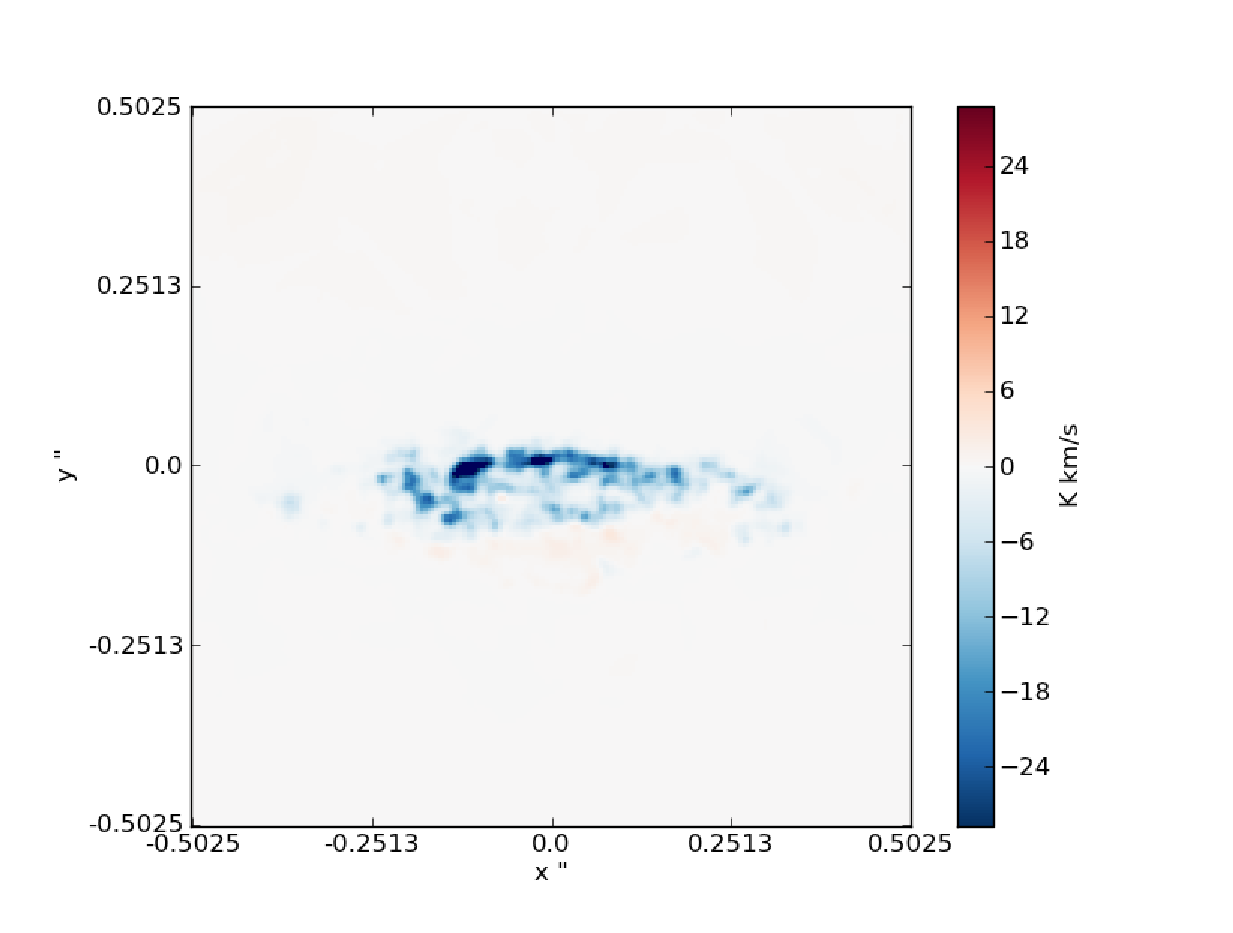
\includegraphics[width=84mm]{Figures/sim/imageC18O_3-2_15deg_contSub.eps}

 \caption{C18O 3-2 15 deg Continuum subtracted mom0}
\end{figure}

%\begin{figure}
% 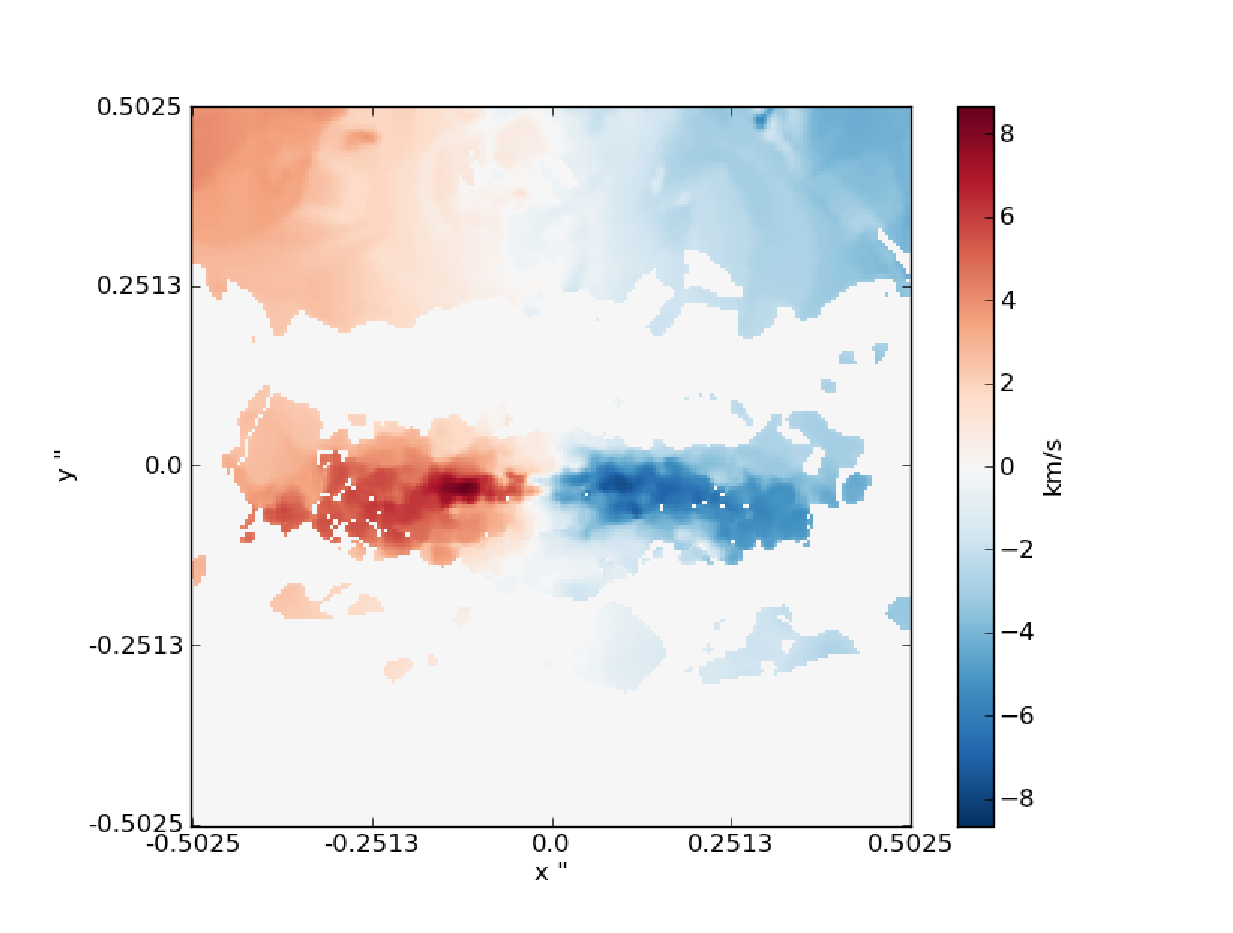
\includegraphics[width=84mm]{Figures/sim/imageC18O_3-2_15deg_mom1.eps}
%
% \caption{C18O 3-2 15 deg mom1map}
%\end{figure}

\begin{figure}
 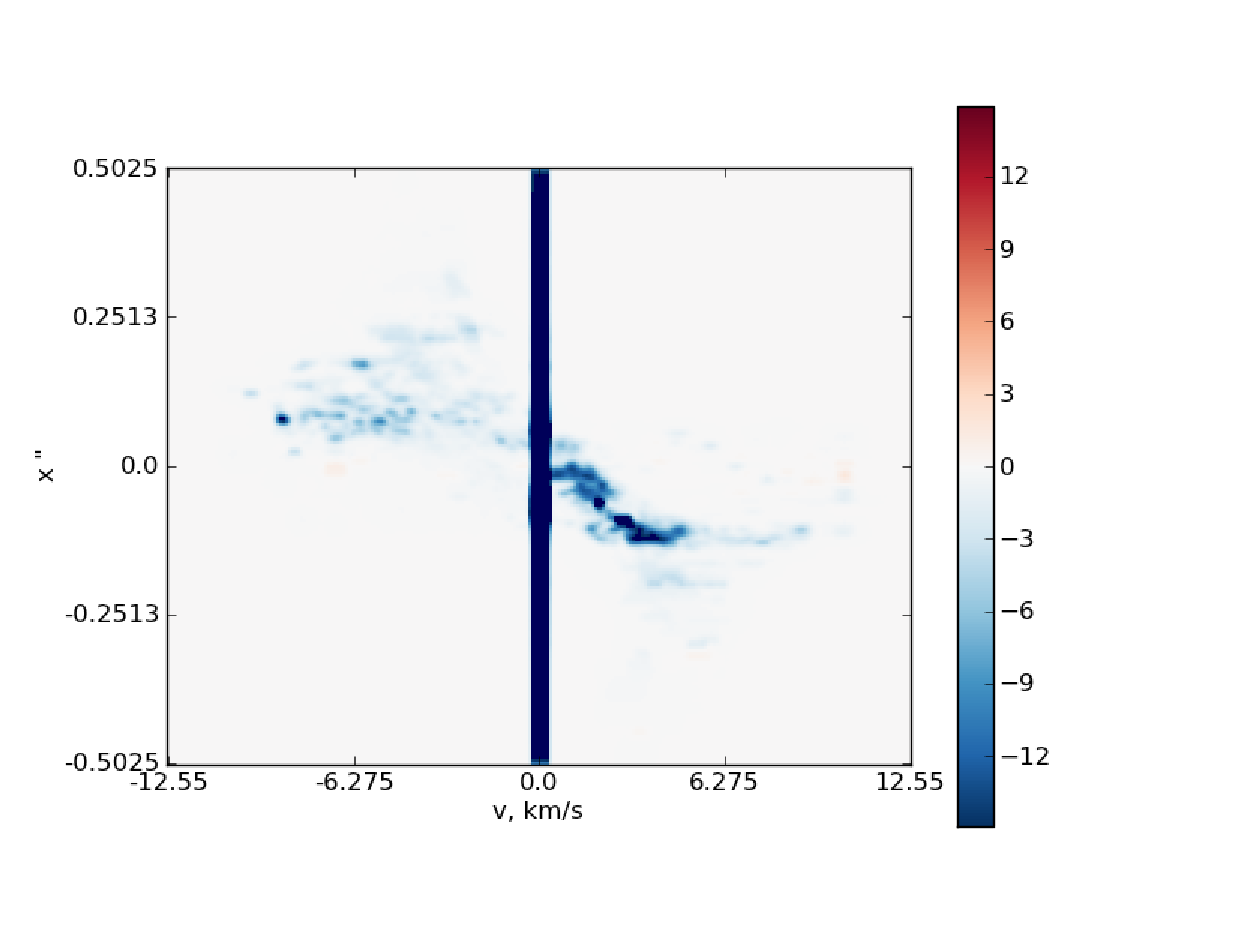
\includegraphics[width=84mm]{Figures/sim/imageC18O_3-2_15deg_PV_centre.eps}

 \caption{C18O 3-2 PV 15 deg through centre}
\end{figure}


\begin{figure}
 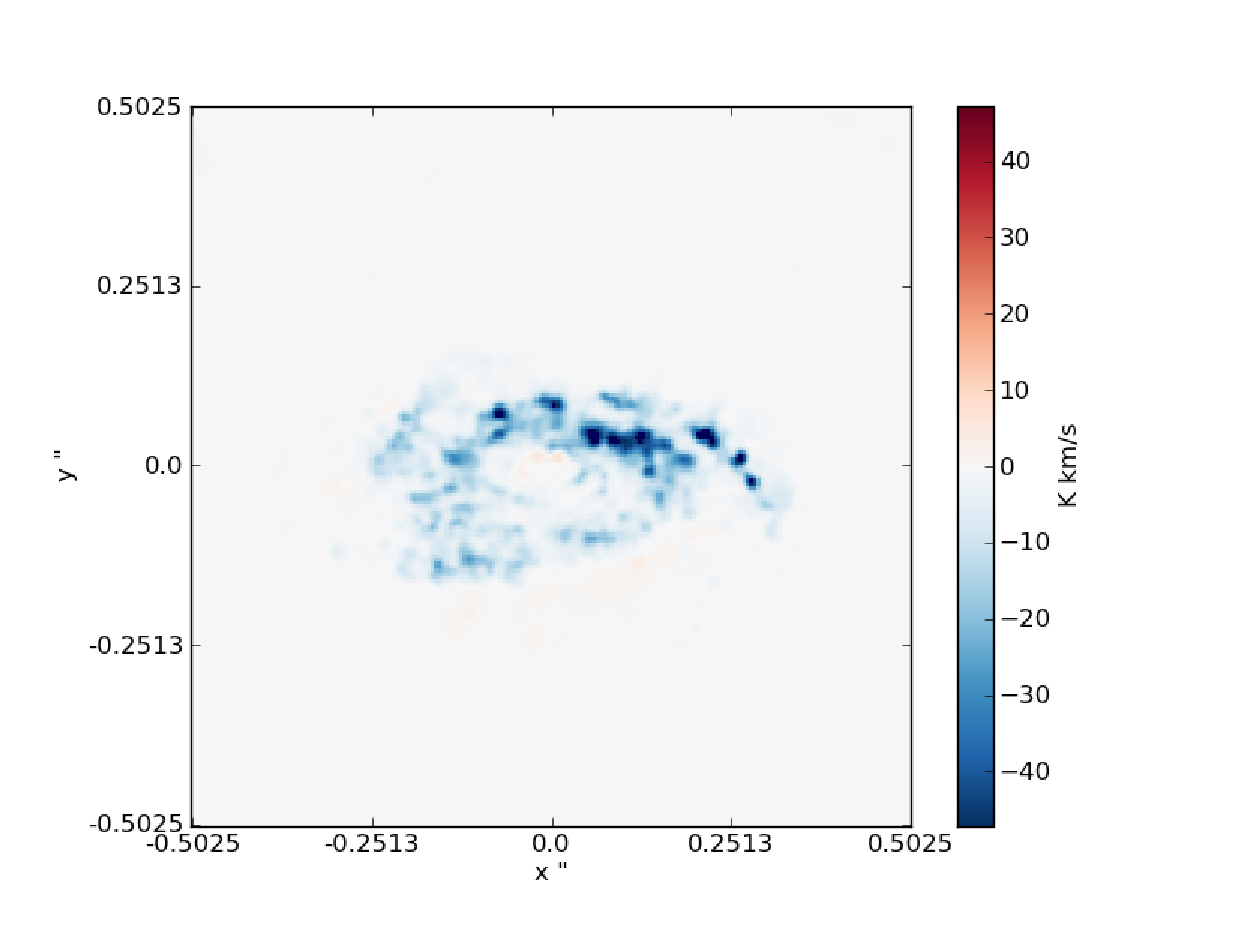
\includegraphics[width=84mm]{Figures/sim/imageC18O_3-2_30deg_contSub.eps}

 \caption{C18O 3-2  30 deg Continuum subtracted mom0}
\end{figure}




%\begin{figure}
% 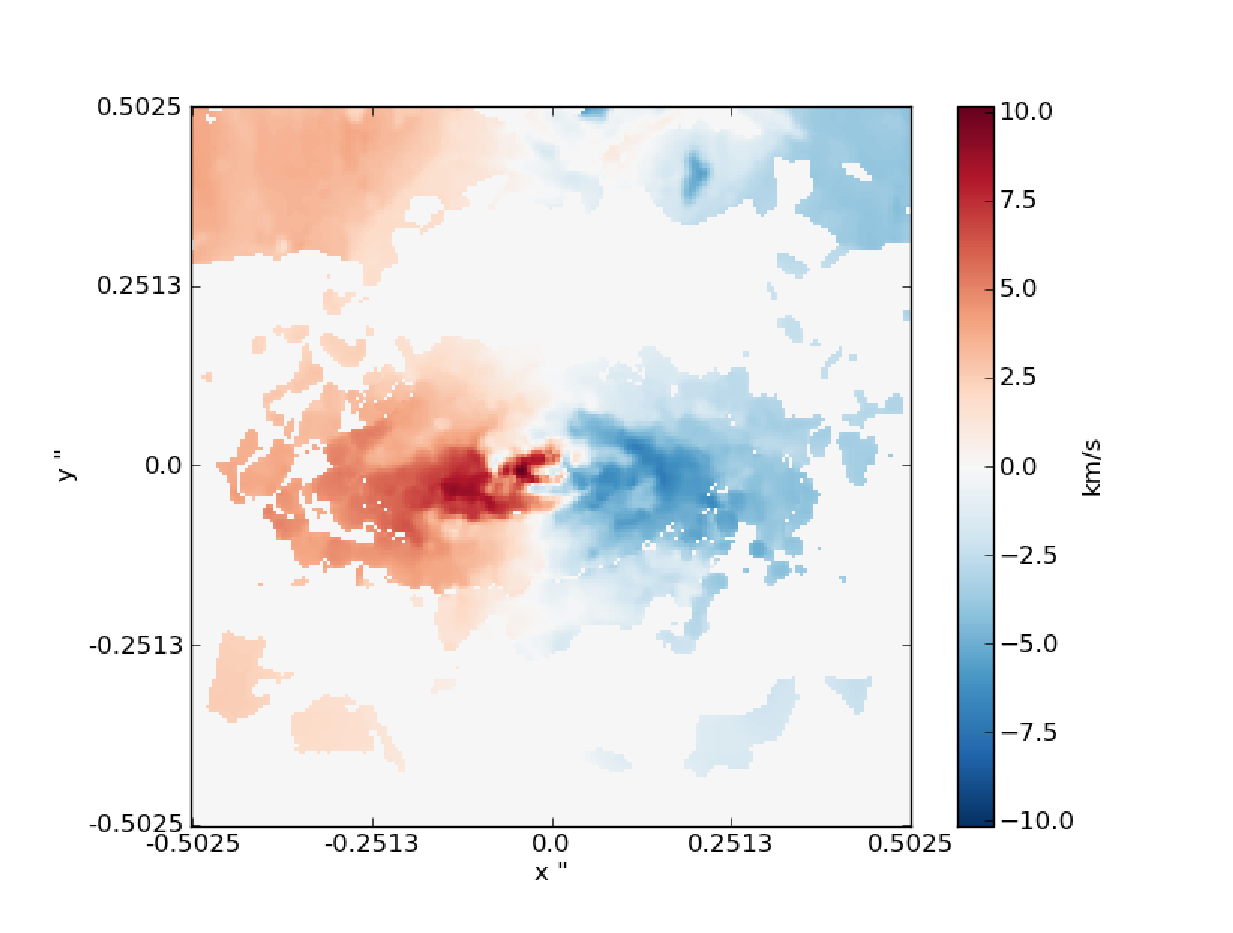
\includegraphics[width=84mm]{Figures/sim/imageC18O_3-2_30deg_mom1.eps}
%
% \caption{C18O 3-2 30 deg mom1map}
%\end{figure}

\begin{figure}
 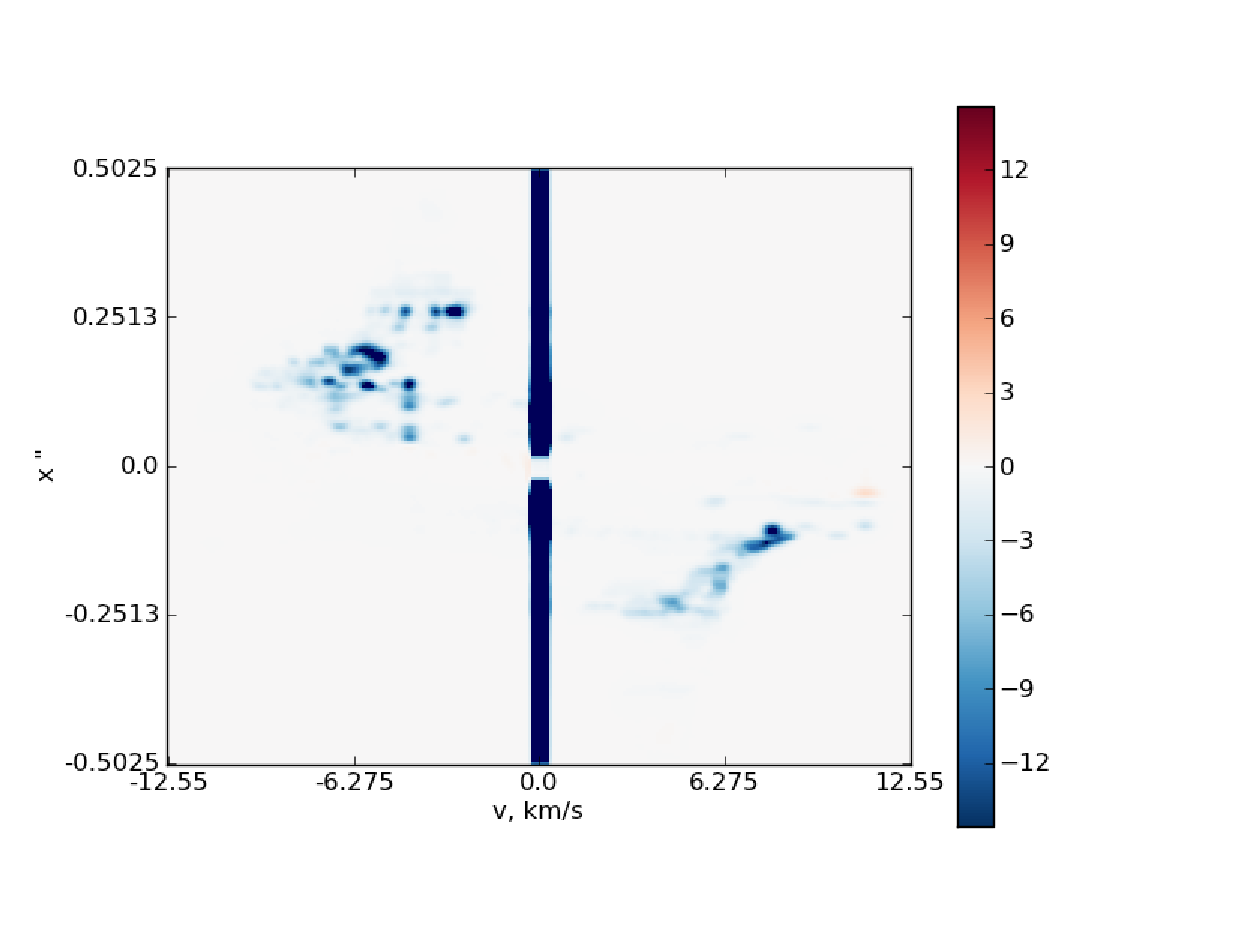
\includegraphics[width=84mm]{Figures/sim/imageC18O_3-2_30deg_PV_centre.eps}

 \caption{C18O 3-2 30 deg PV through centre}
\end{figure}

\begin{figure}
 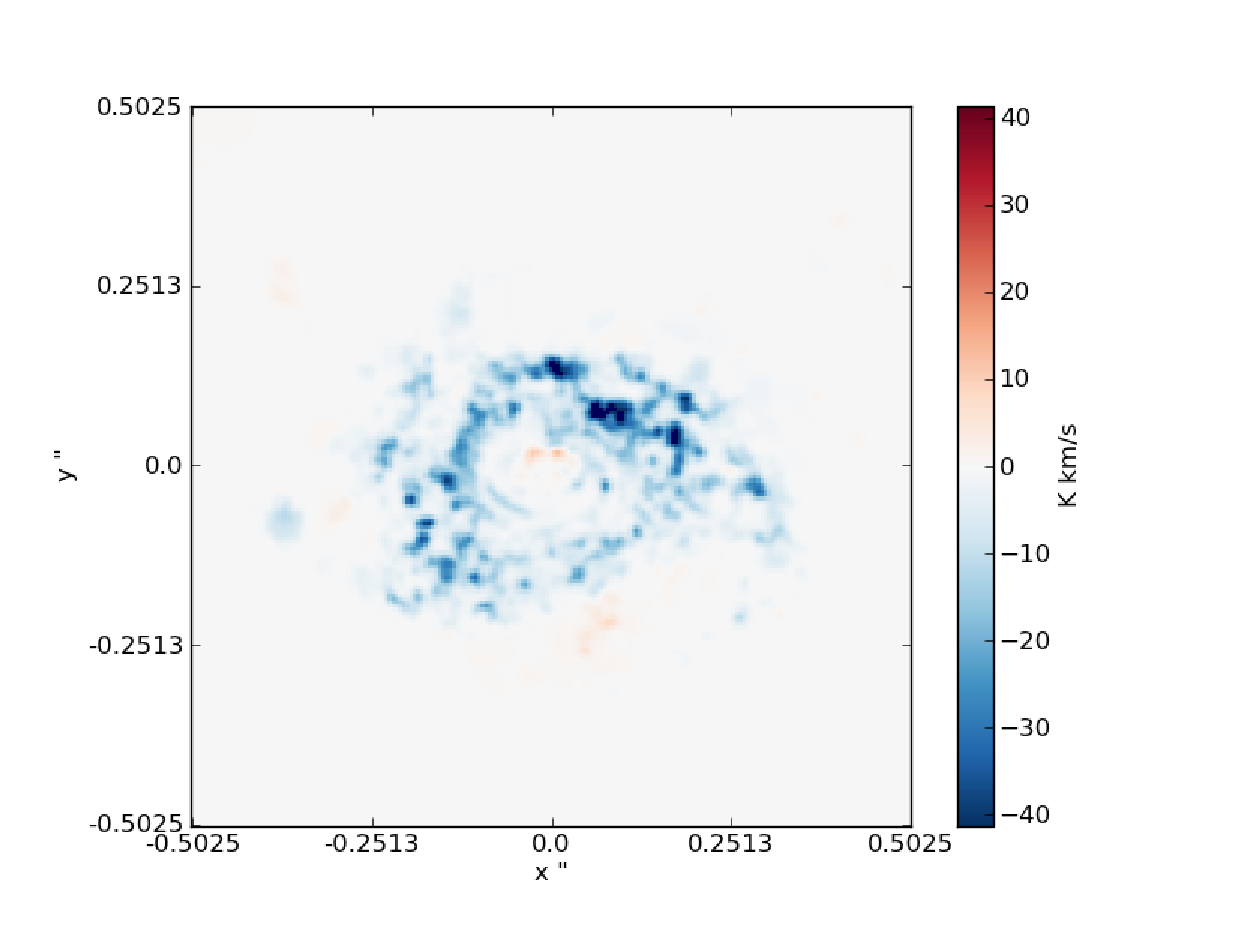
\includegraphics[width=84mm]{Figures/sim/imageC18O_3-2_45deg_contSub.eps}

 \caption{C18O 3-2 45 deg Continuum subtracted mom0}
\end{figure}

%\begin{figure}
% 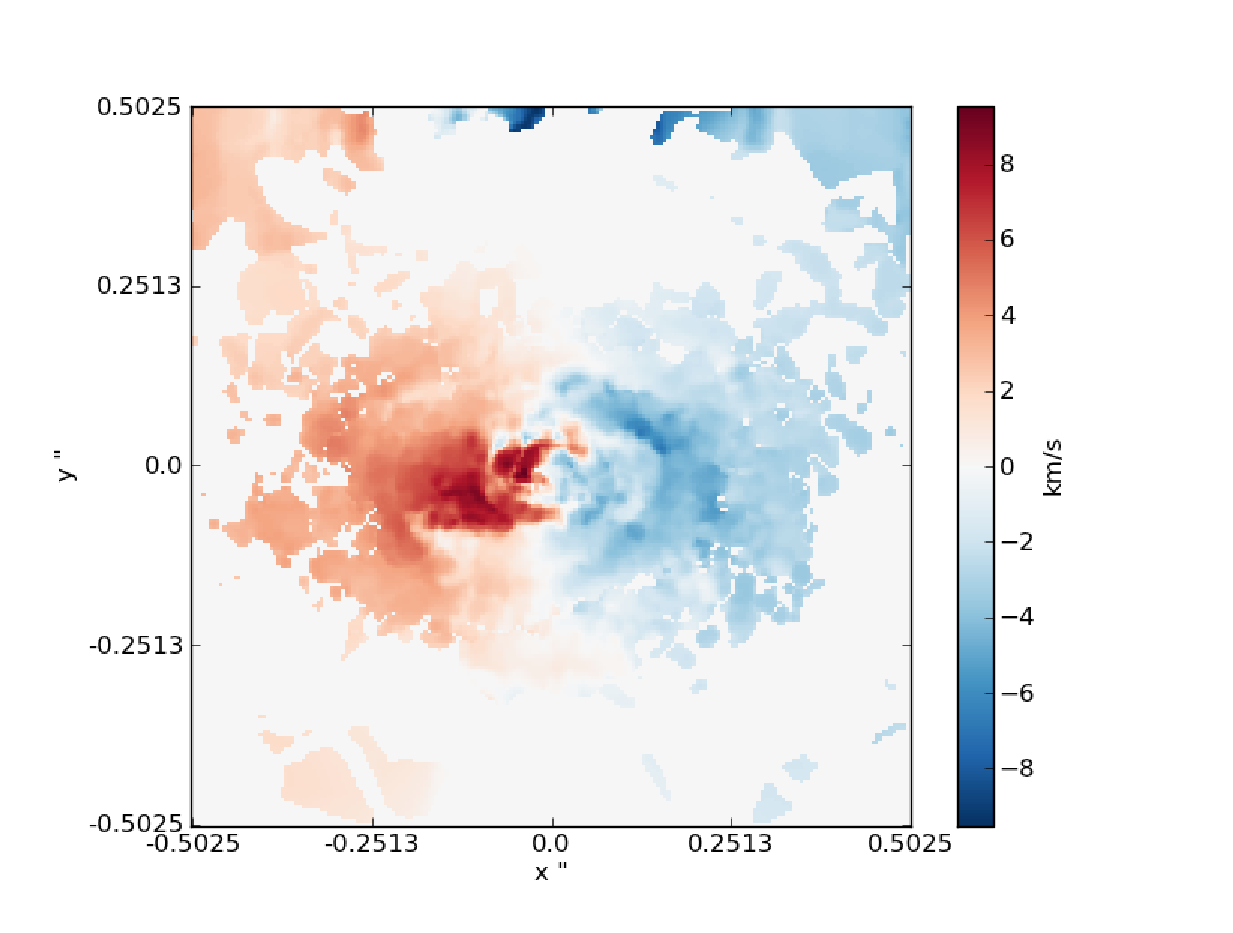
\includegraphics[width=84mm]{Figures/sim/imageC18O_3-2_45deg_mom1.eps}
%
% \caption{C18O 3-2 45 deg mom1map}
%\end{figure}

\begin{figure}
 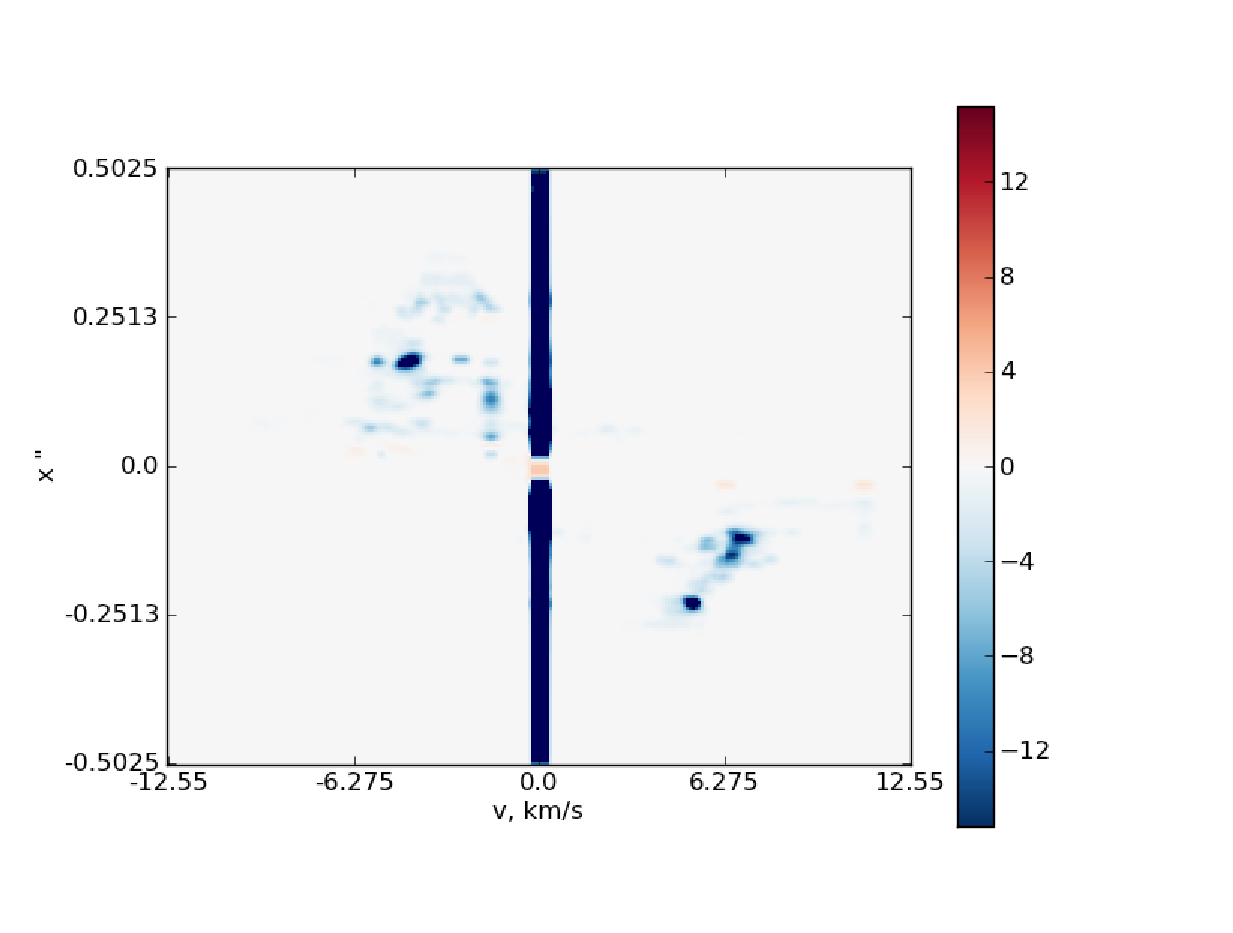
\includegraphics[width=84mm]{Figures/sim/imageC18O_3-2_45deg_PV_centre.eps}

 \caption{C18O 3-2 45 deg PV through centre}
\end{figure}


\begin{figure}
 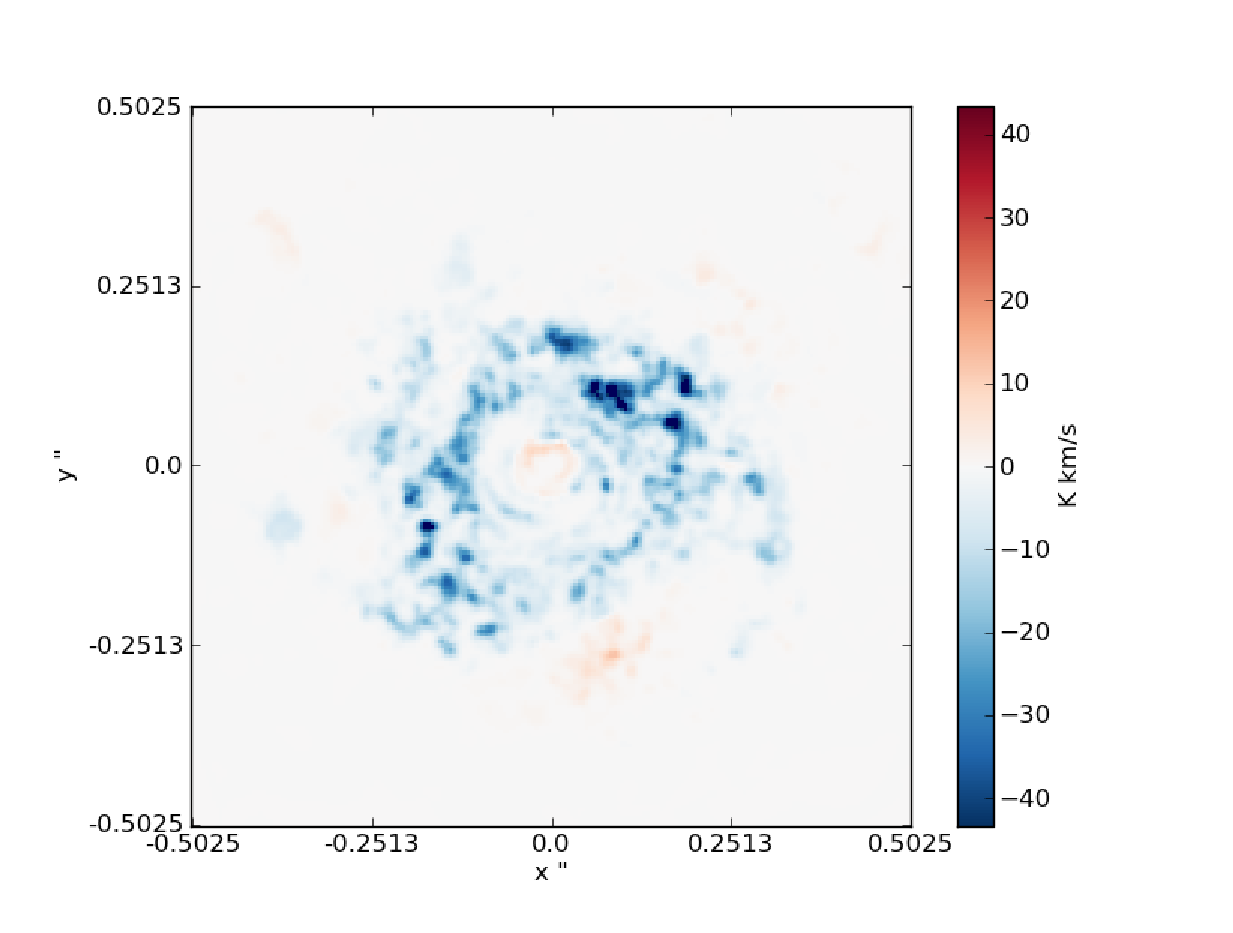
\includegraphics[width=84mm]{Figures/sim/imageC18O_3-2_60deg_contSub.eps}

 \caption{C18O 3-2 60 deg Continuum subtracted mom0}
\end{figure}

%\begin{figure}
% 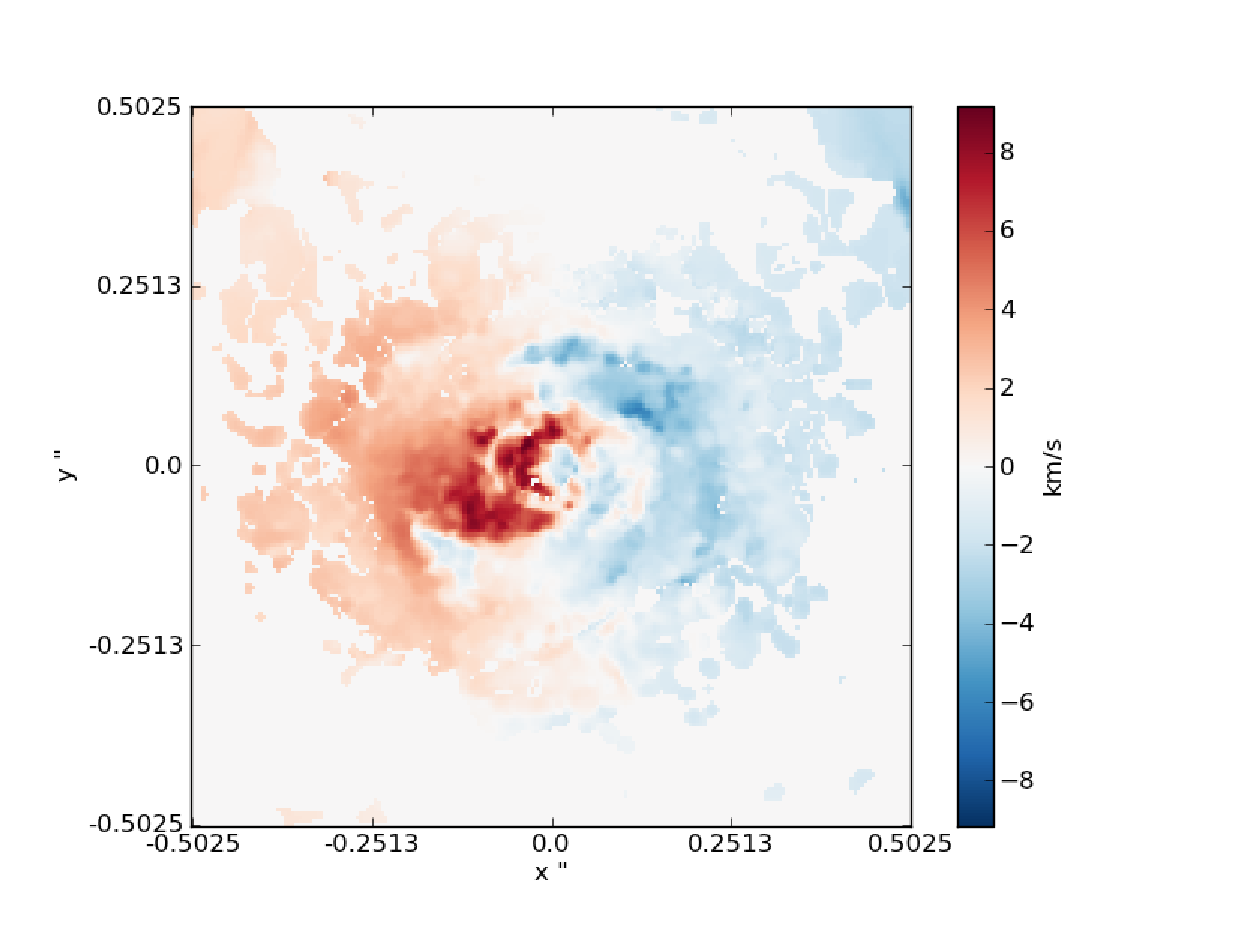
\includegraphics[width=84mm]{Figures/sim/imageC18O_3-2_60deg_mom1.eps}
%
% \caption{C18O 3-2 60 deg mom1map}
%\end{figure}

\begin{figure}
 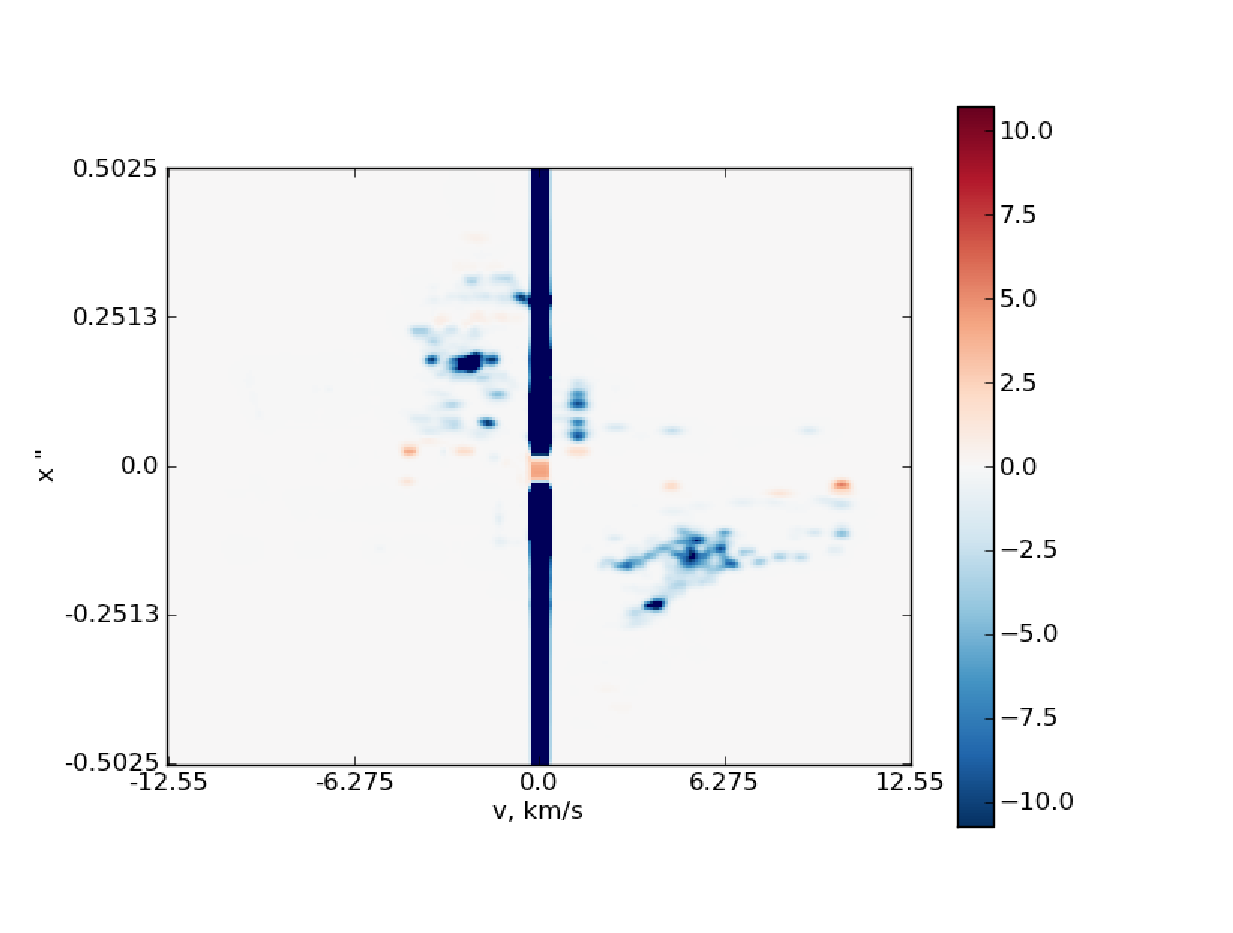
\includegraphics[width=84mm]{Figures/sim/imageC18O_3-2_60deg_PV_centre.eps}

 \caption{C18O 3-2 60 deg PV through centre}
\end{figure}

\begin{figure}
 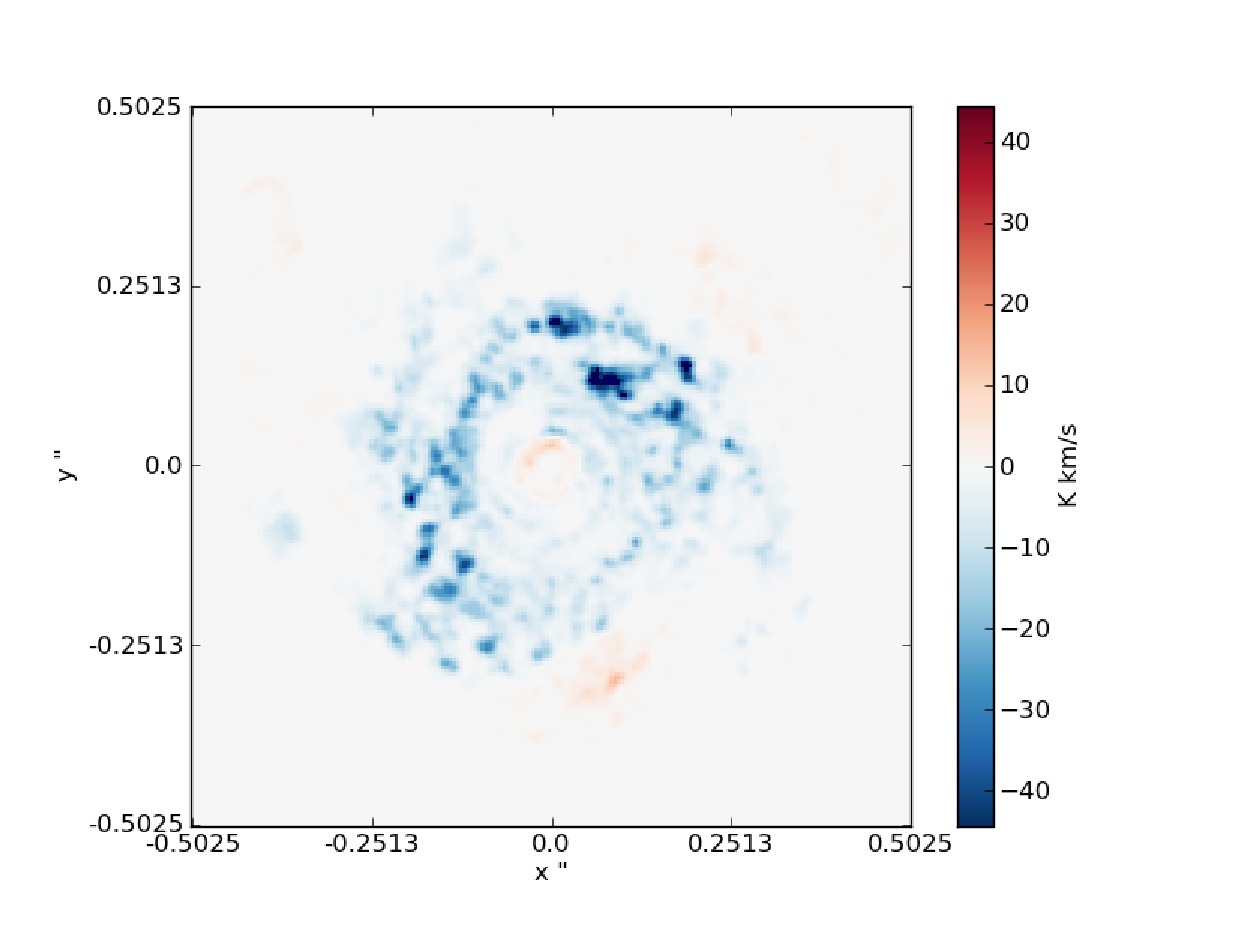
\includegraphics[width=84mm]{Figures/sim/imageC18O_3-2_75deg_contSub.eps}

 \caption{C18O 3-2 75 deg Continuum subtracted mom0}
\end{figure}

%\begin{figure}
% 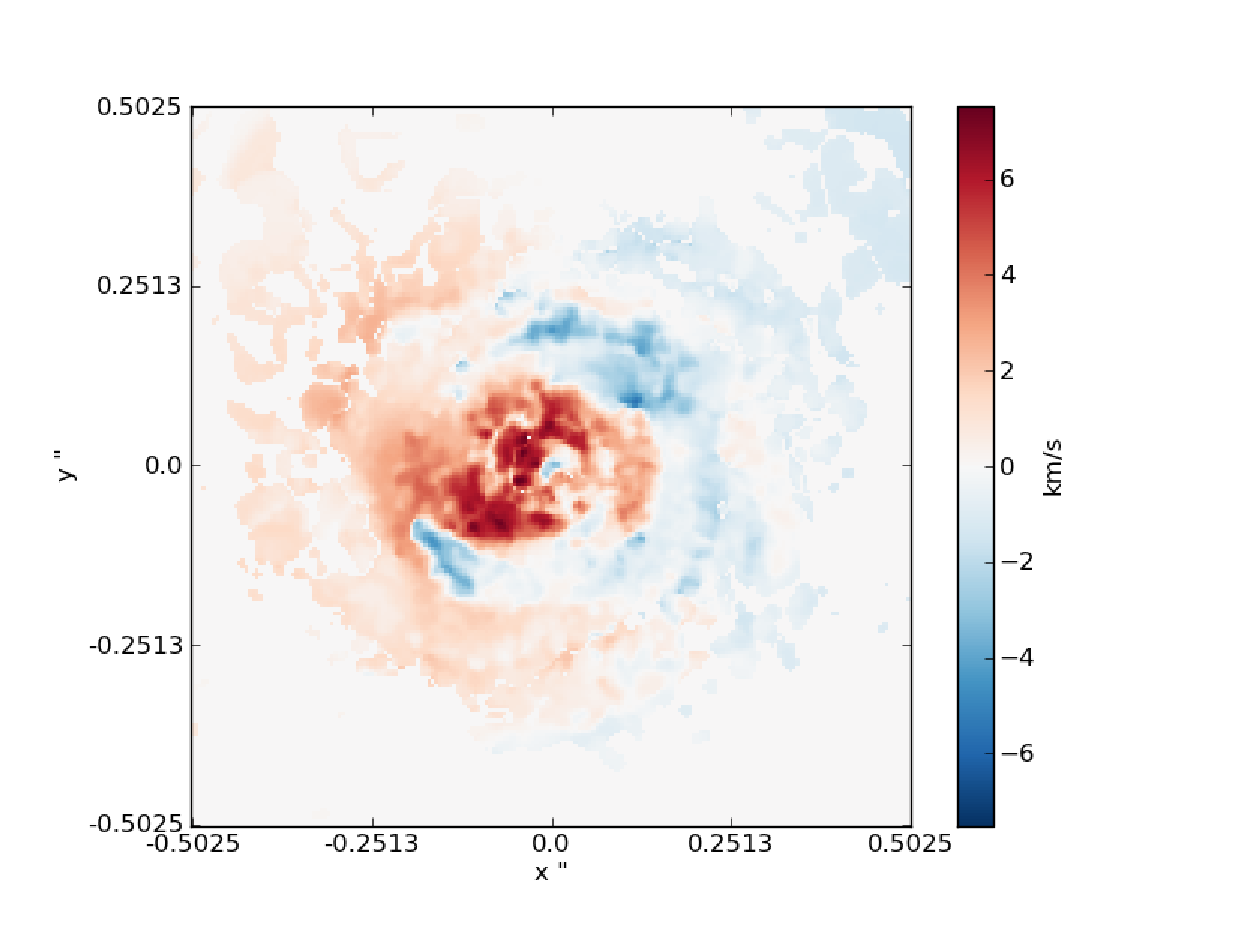
\includegraphics[width=84mm]{Figures/sim/imageC18O_3-2_75deg_mom1.eps}
%
% \caption{C18O 3-2 75 deg mom1map}
%\end{figure}

\begin{figure}
%  \showthe\columnwidth % Use this to determine the width of the figure.
  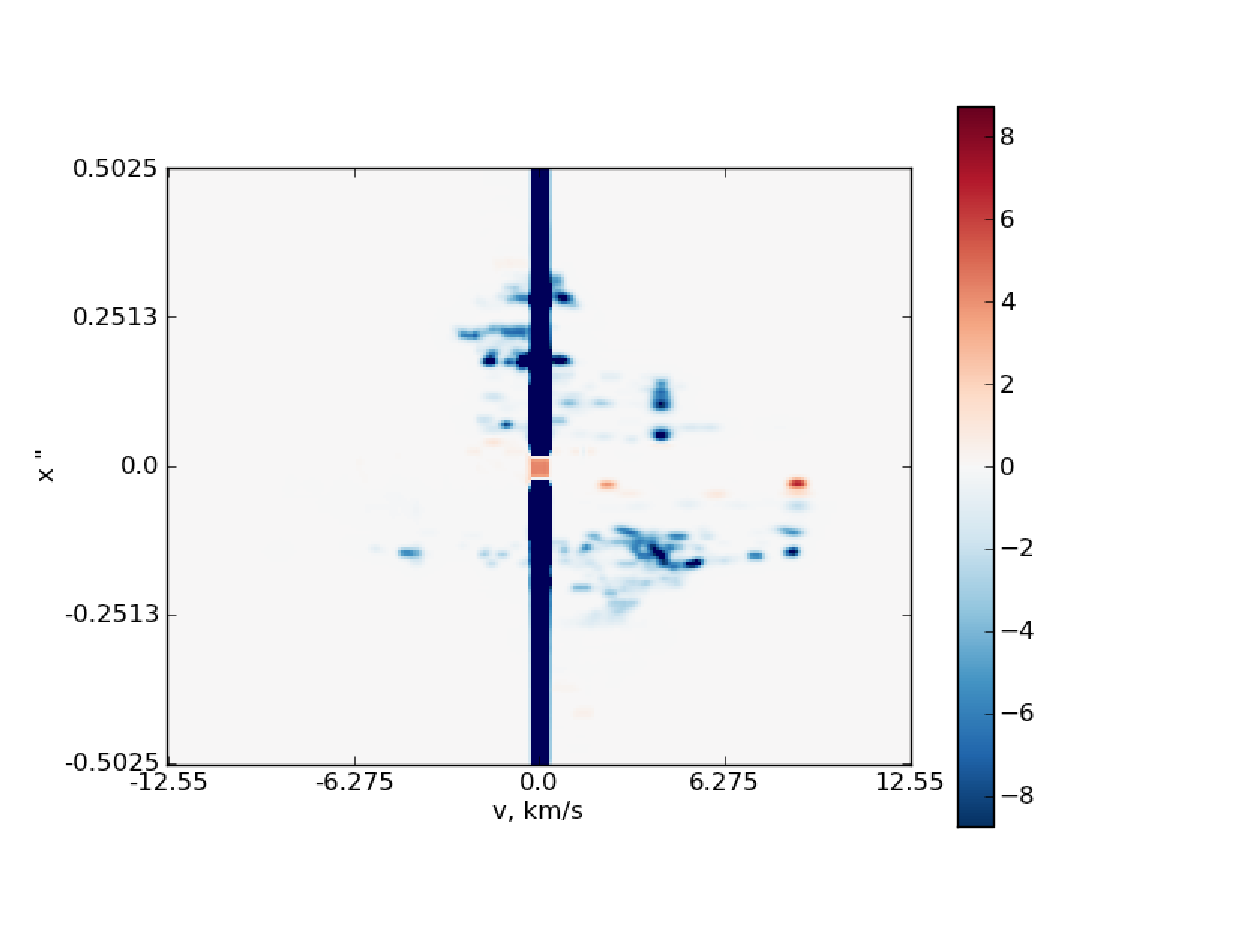
\includegraphics[width=84mm]{Figures/sim/imageC18O_3-2_75deg_PV_centre.eps}
  \caption{C18O 3-2 75 deg PV through centre}
\end{figure}

\bsp
%
\label{lastpage}
%
\end{document}
